\section{レポート課題1}
\subsection{課題1}
ロジスティク写像の時系列変化を計算するプログラムを作成し、$r = 1.50, r = 2.60,r = 3.20, r = 3.50,$ \\
$r = 3.86, r = 3.90 のとき、x0 = 0.7$として個体数変動の時系列グラフを表示せよ。\\
画像:\\
\begin{figure}[htbp]
  \begin{tabular}{cc}
    \begin{minipage}[t]{0.45\hsize}
      \centering
      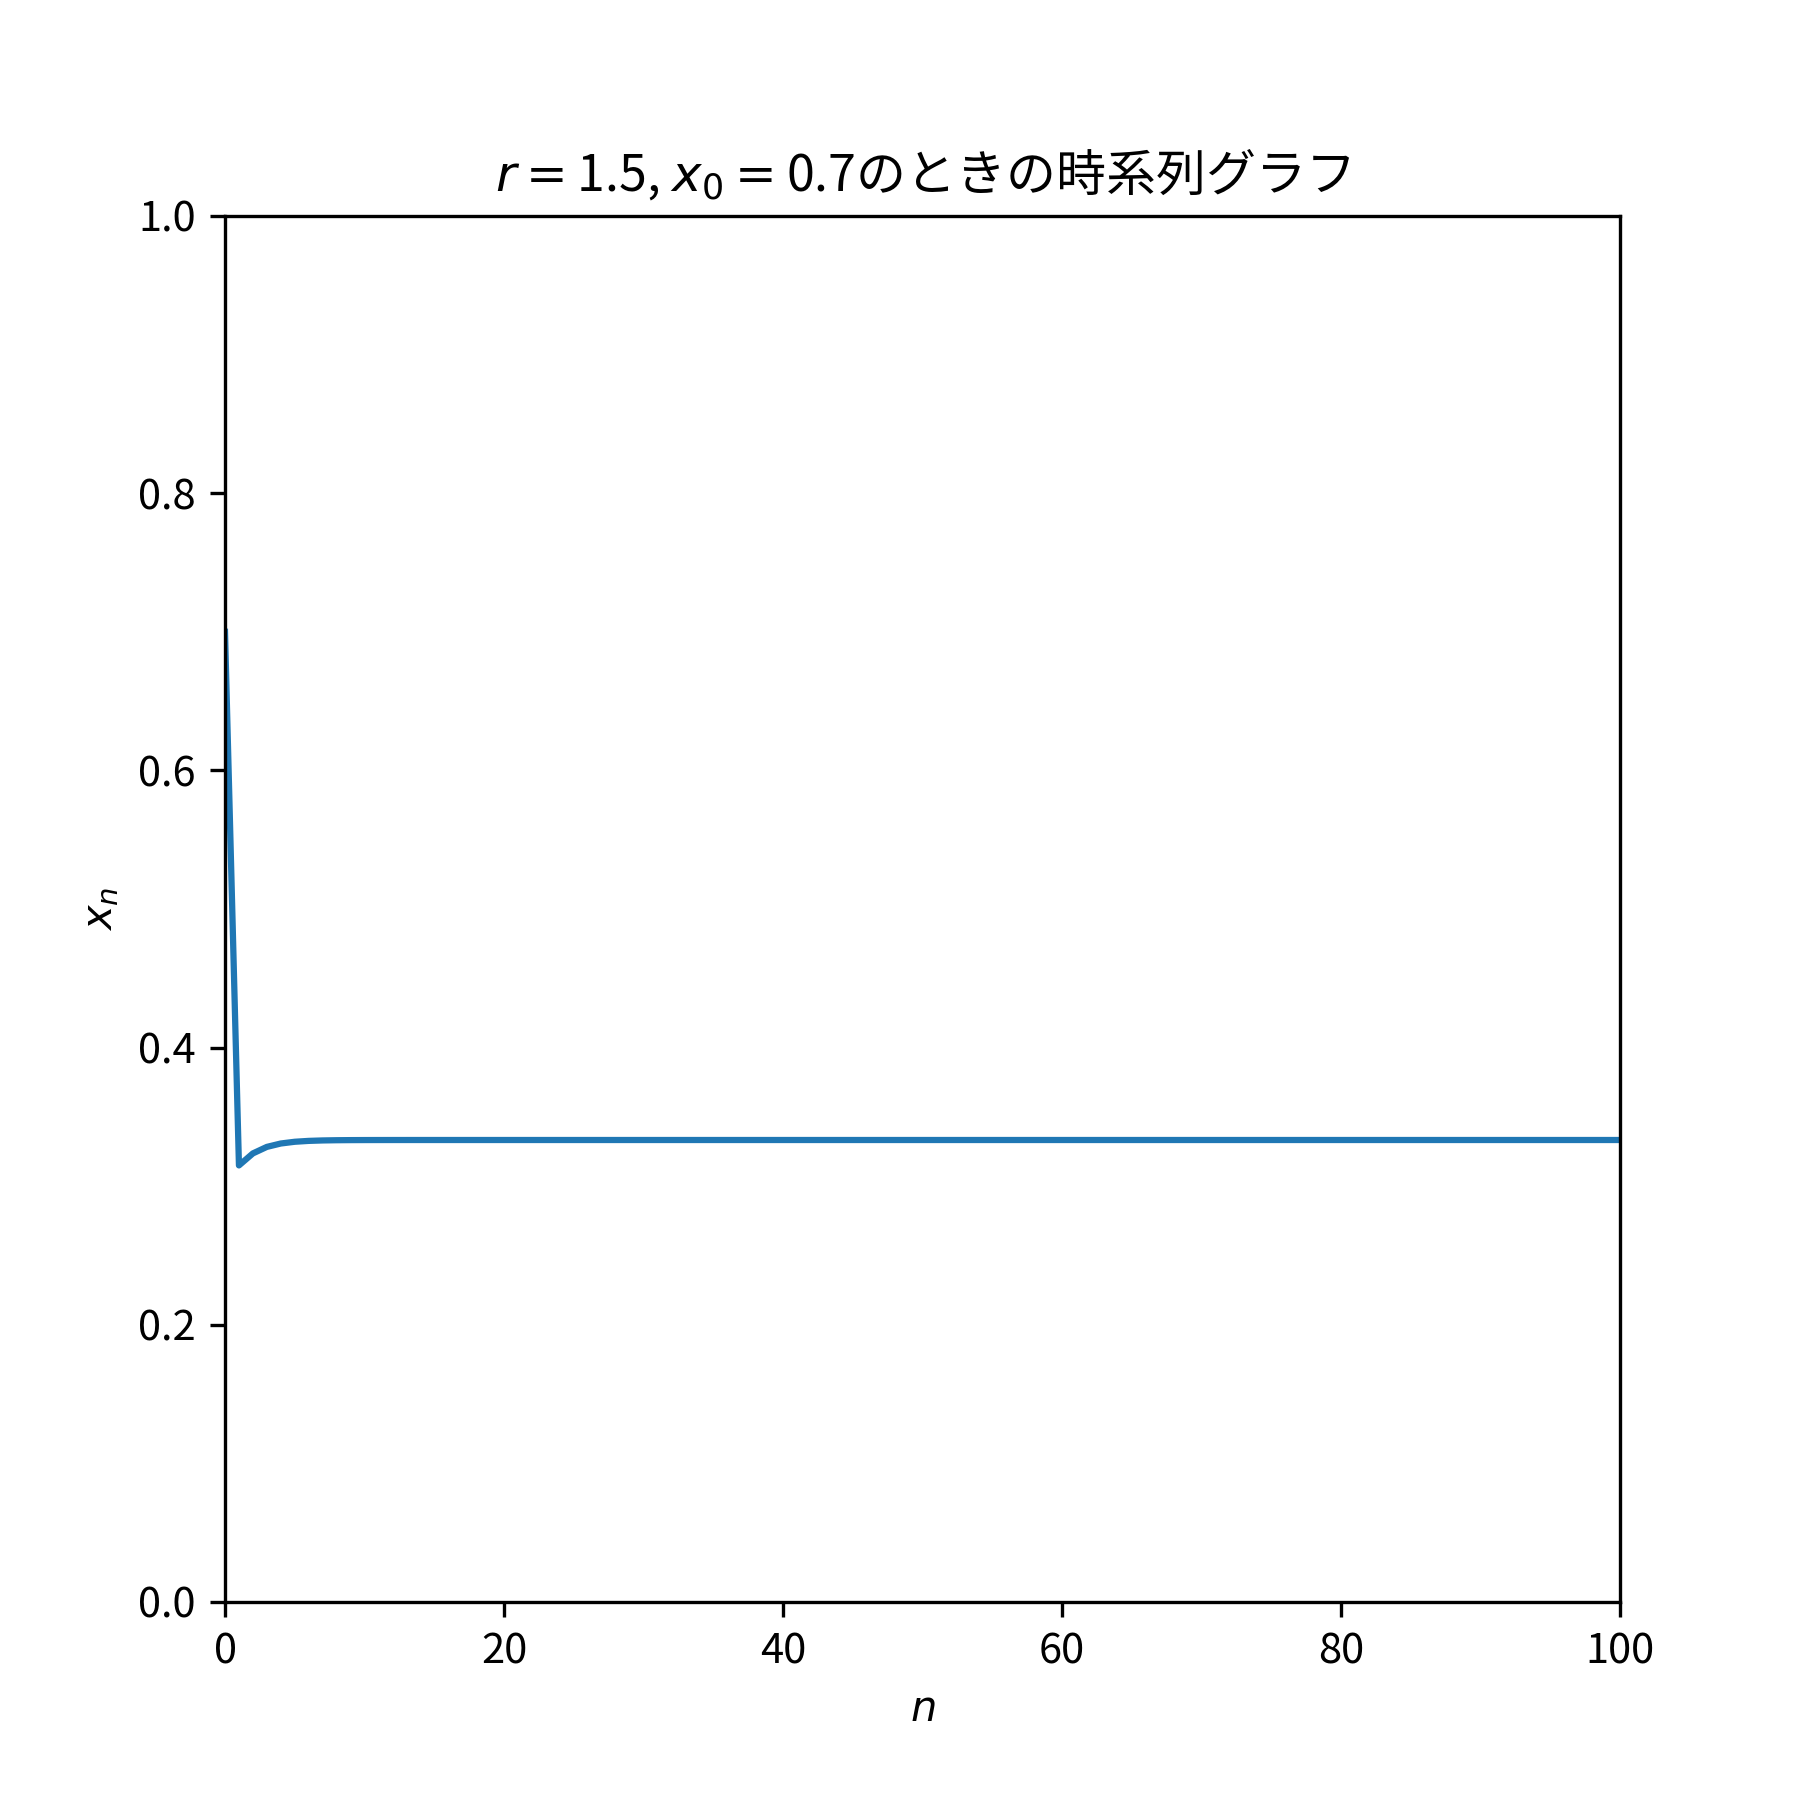
\includegraphics[keepaspectratio, scale=0.3]{images/Problem1/ctest2_1_1.png}
    \end{minipage} &
    \begin{minipage}[t]{0.45\hsize}
      \centering
      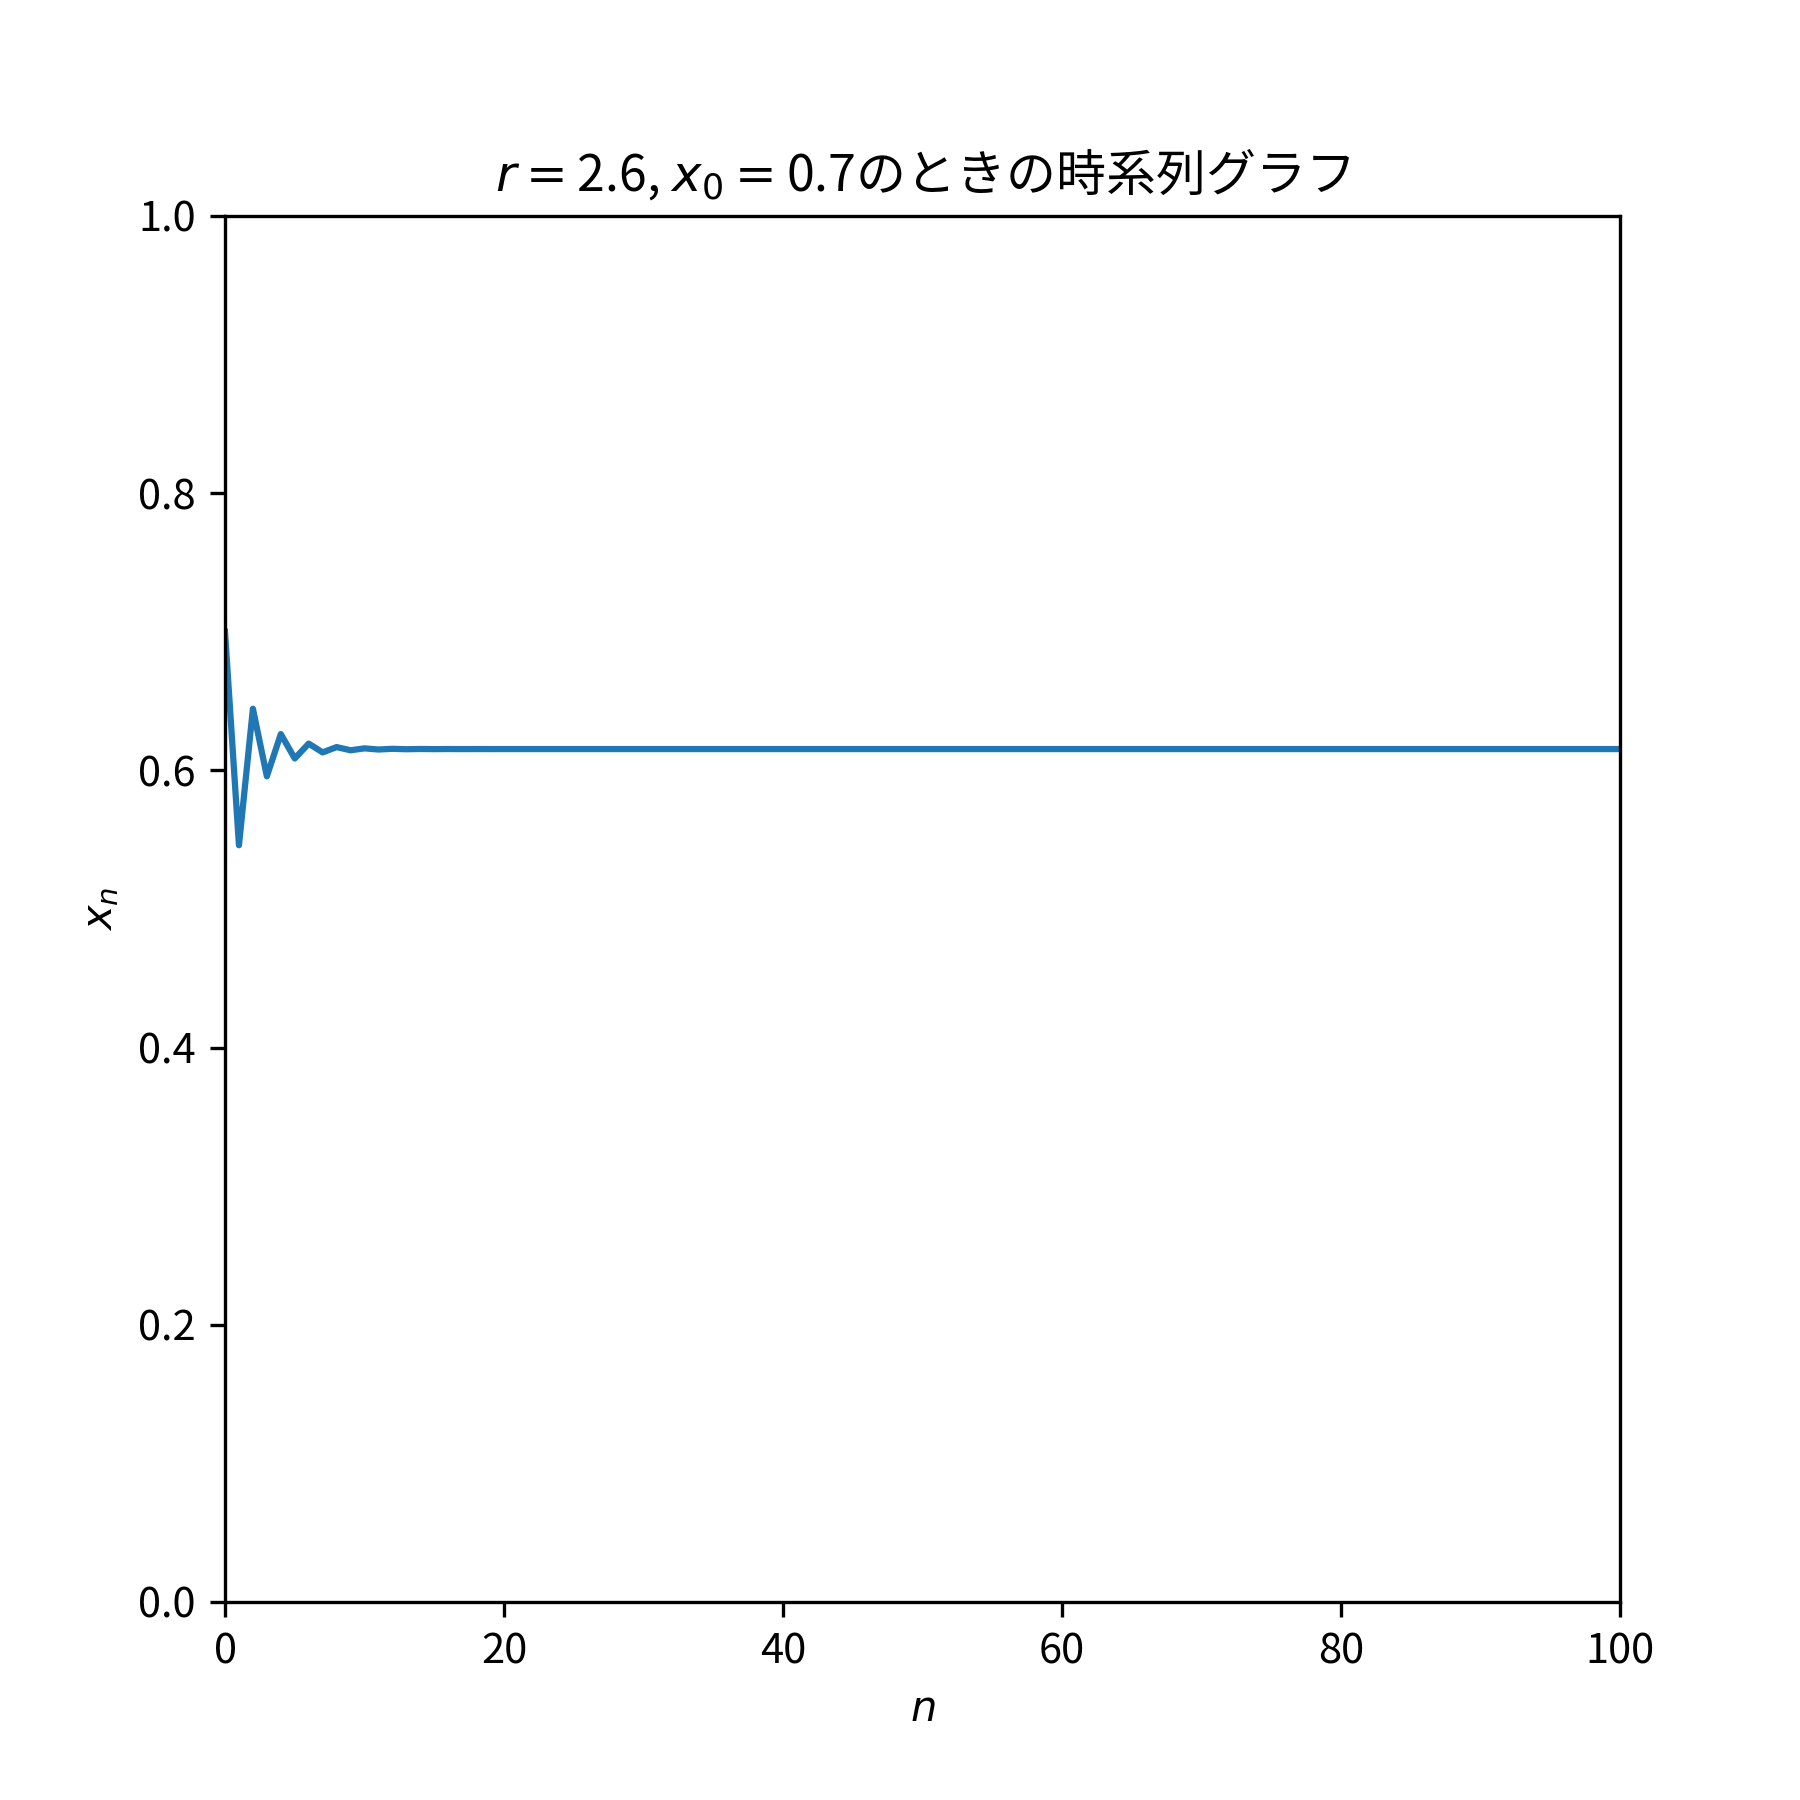
\includegraphics[keepaspectratio, scale=0.3]{images/Problem1/ctest2_2_1.png}
    \end{minipage} \\

    \begin{minipage}[t]{0.45\hsize}
      \centering
      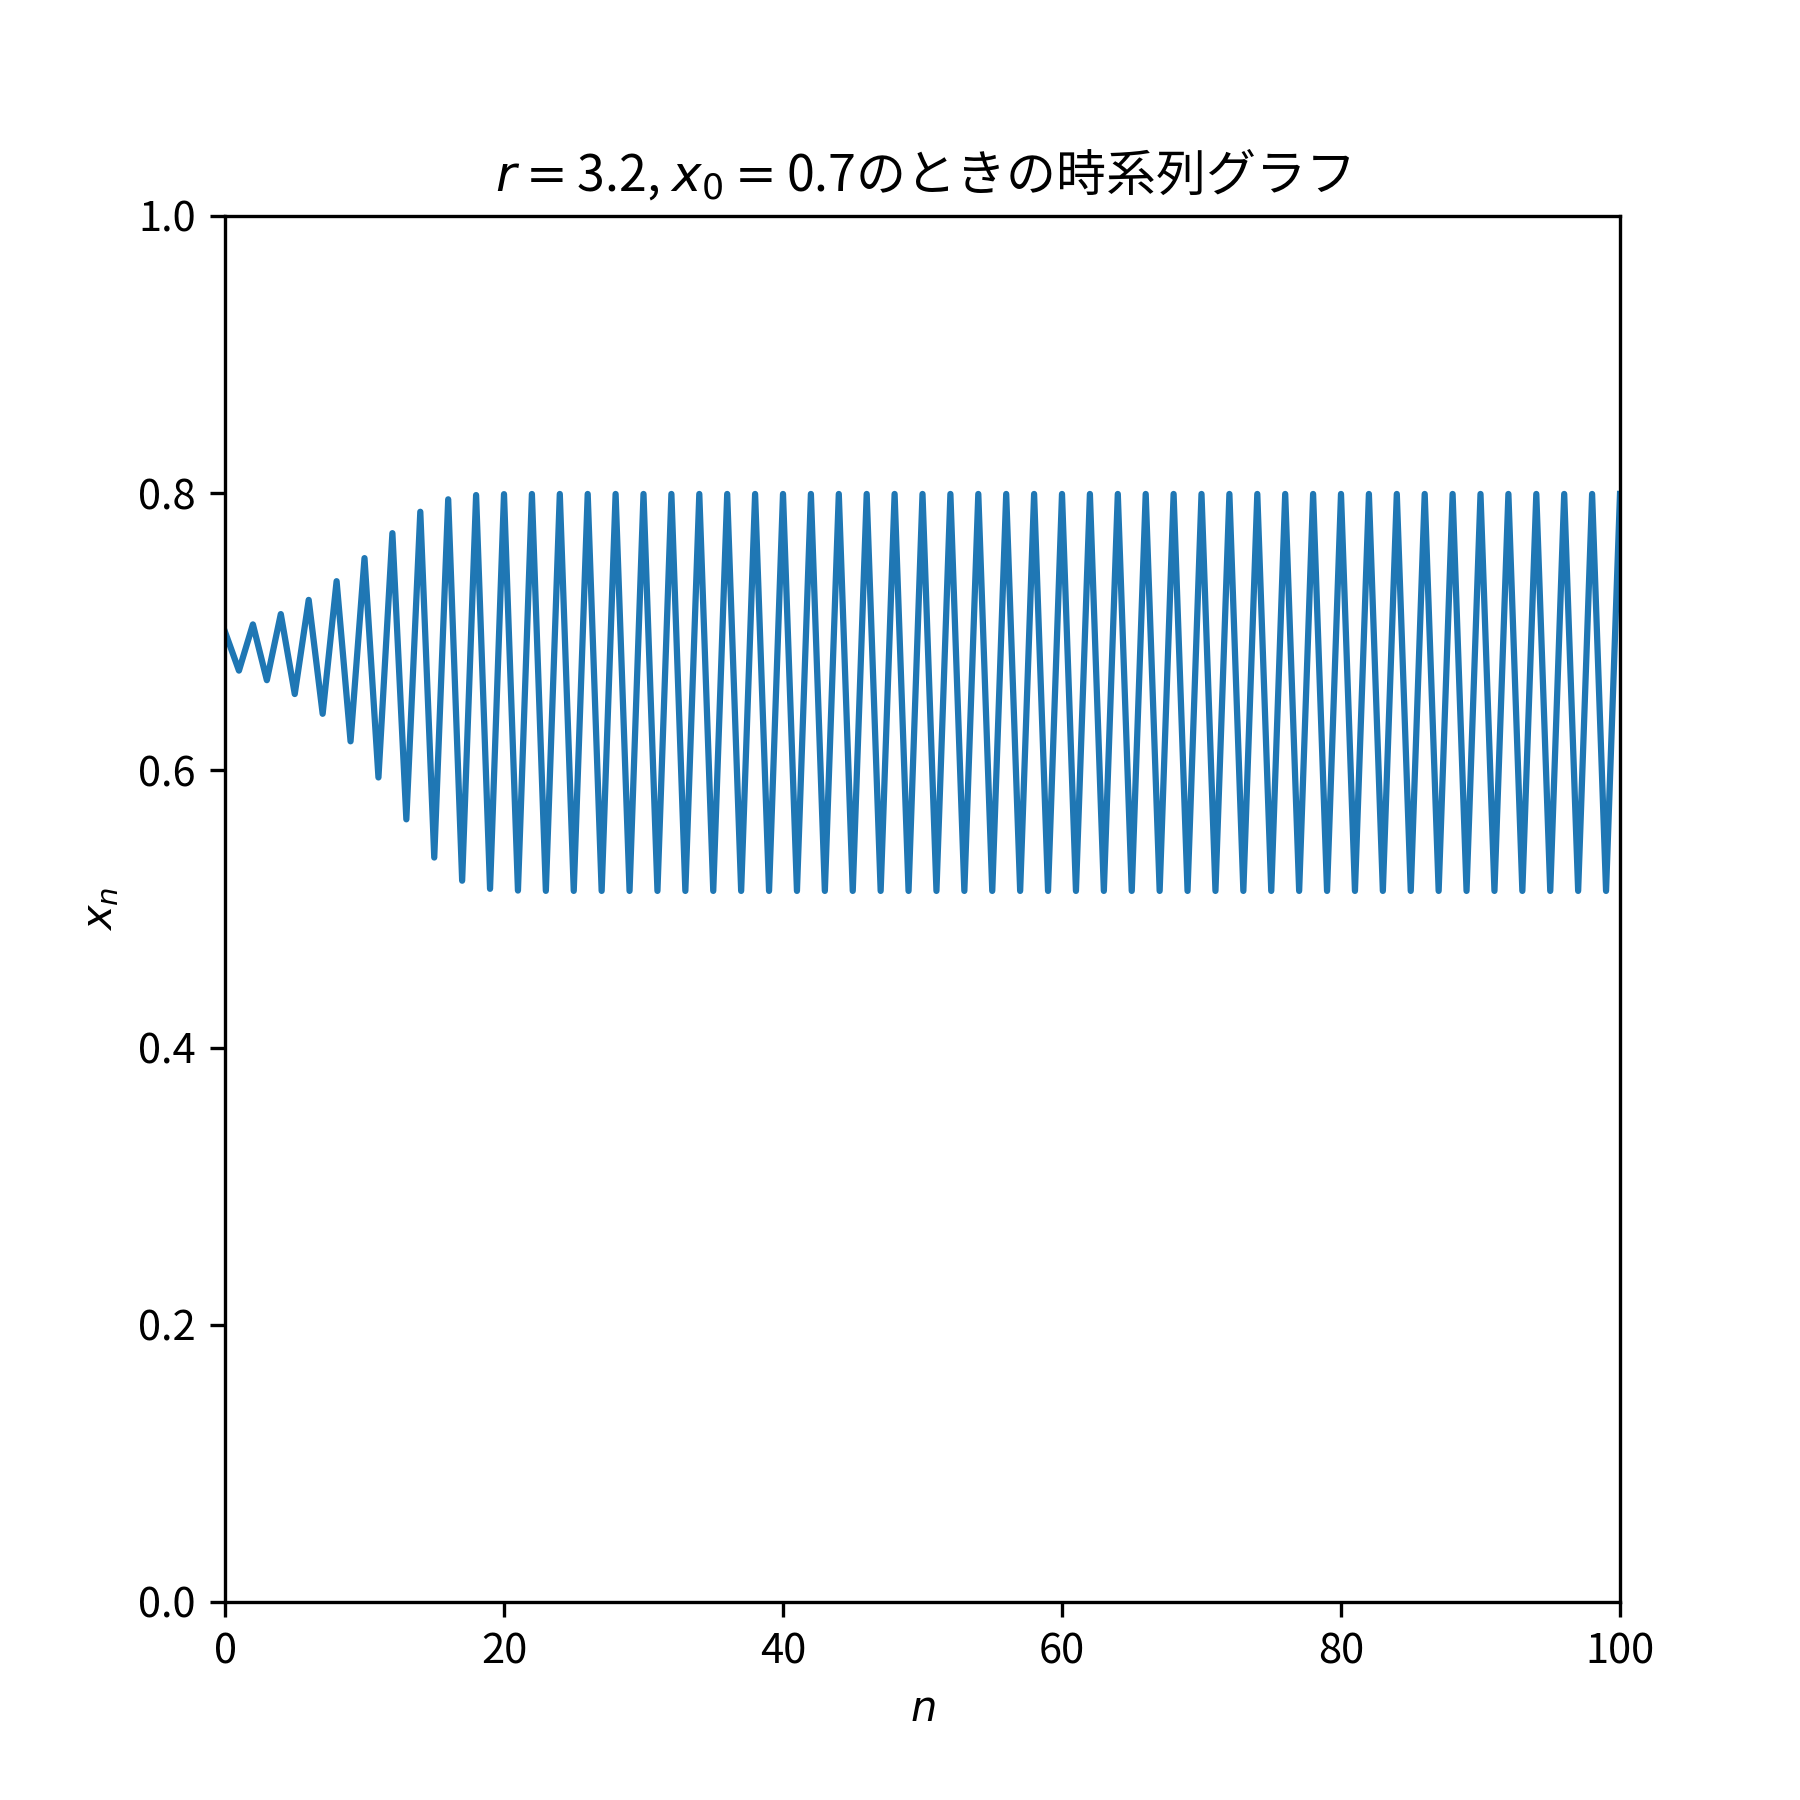
\includegraphics[keepaspectratio, scale=0.3]{images/Problem1/ctest2_3_1.png}
    \end{minipage} &
    \begin{minipage}[t]{0.45\hsize}
      \centering
      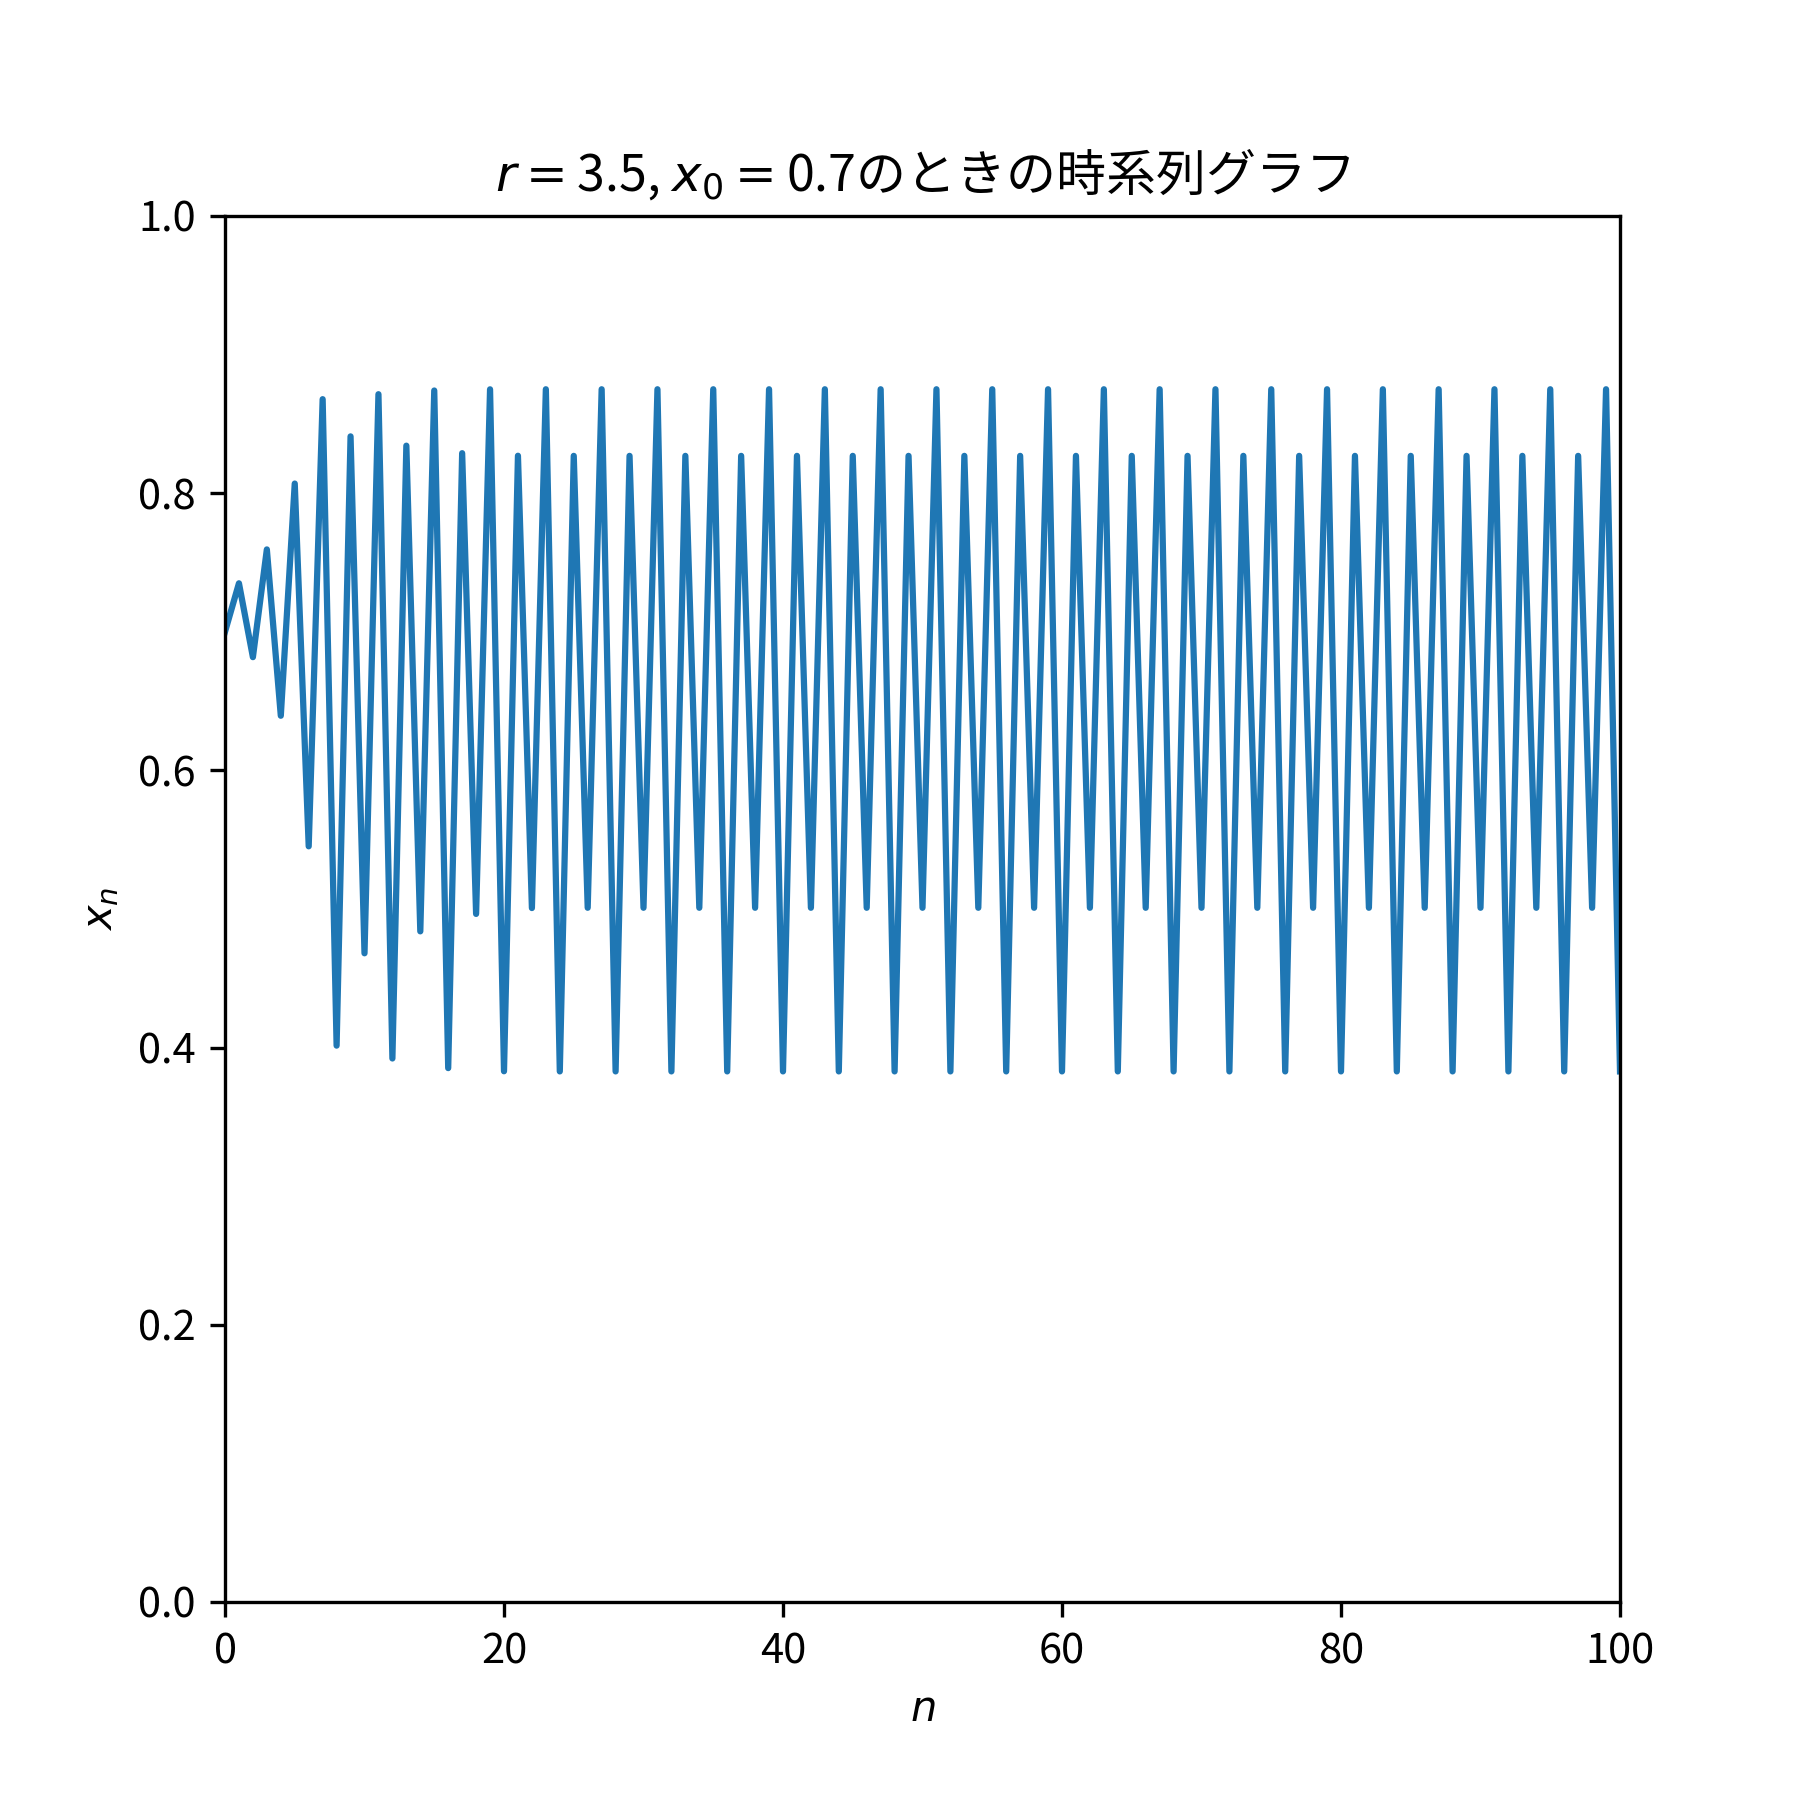
\includegraphics[keepaspectratio, scale=0.3]{images/Problem1/ctest2_4_1.png}
    \end{minipage} \\

    \begin{minipage}[t]{0.45\hsize}
      \centering
      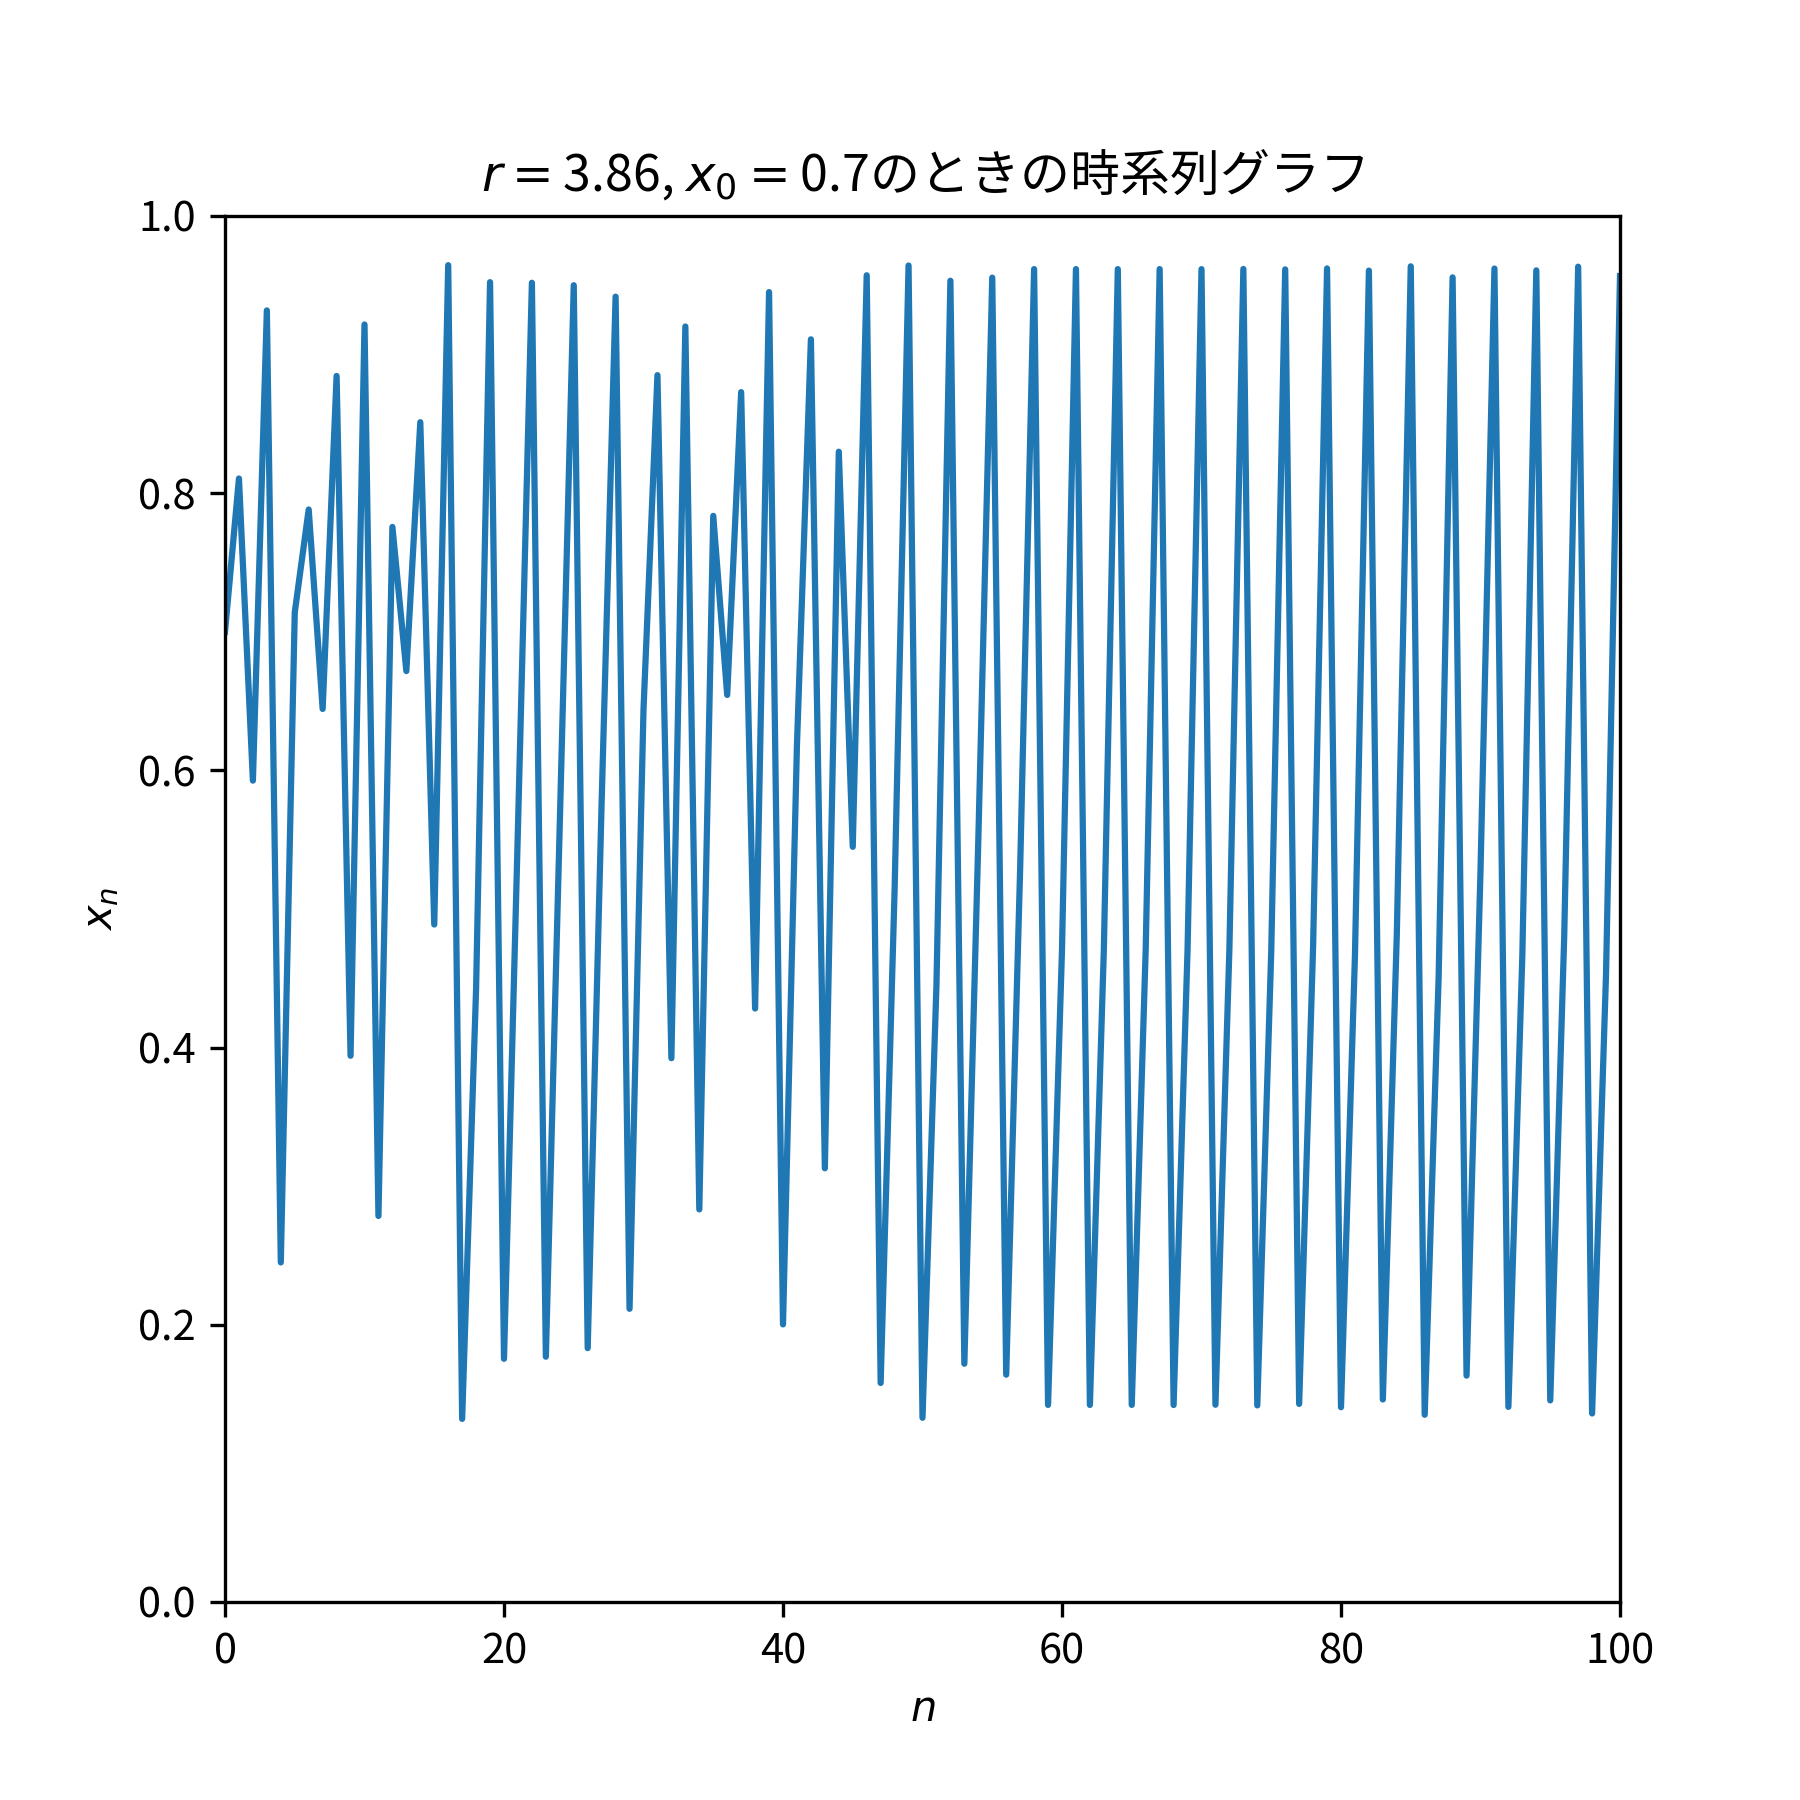
\includegraphics[keepaspectratio, scale=0.3]{images/Problem1/ctest2_5_1.png}
    \end{minipage} &
    \begin{minipage}[t]{0.45\hsize}
      \centering
      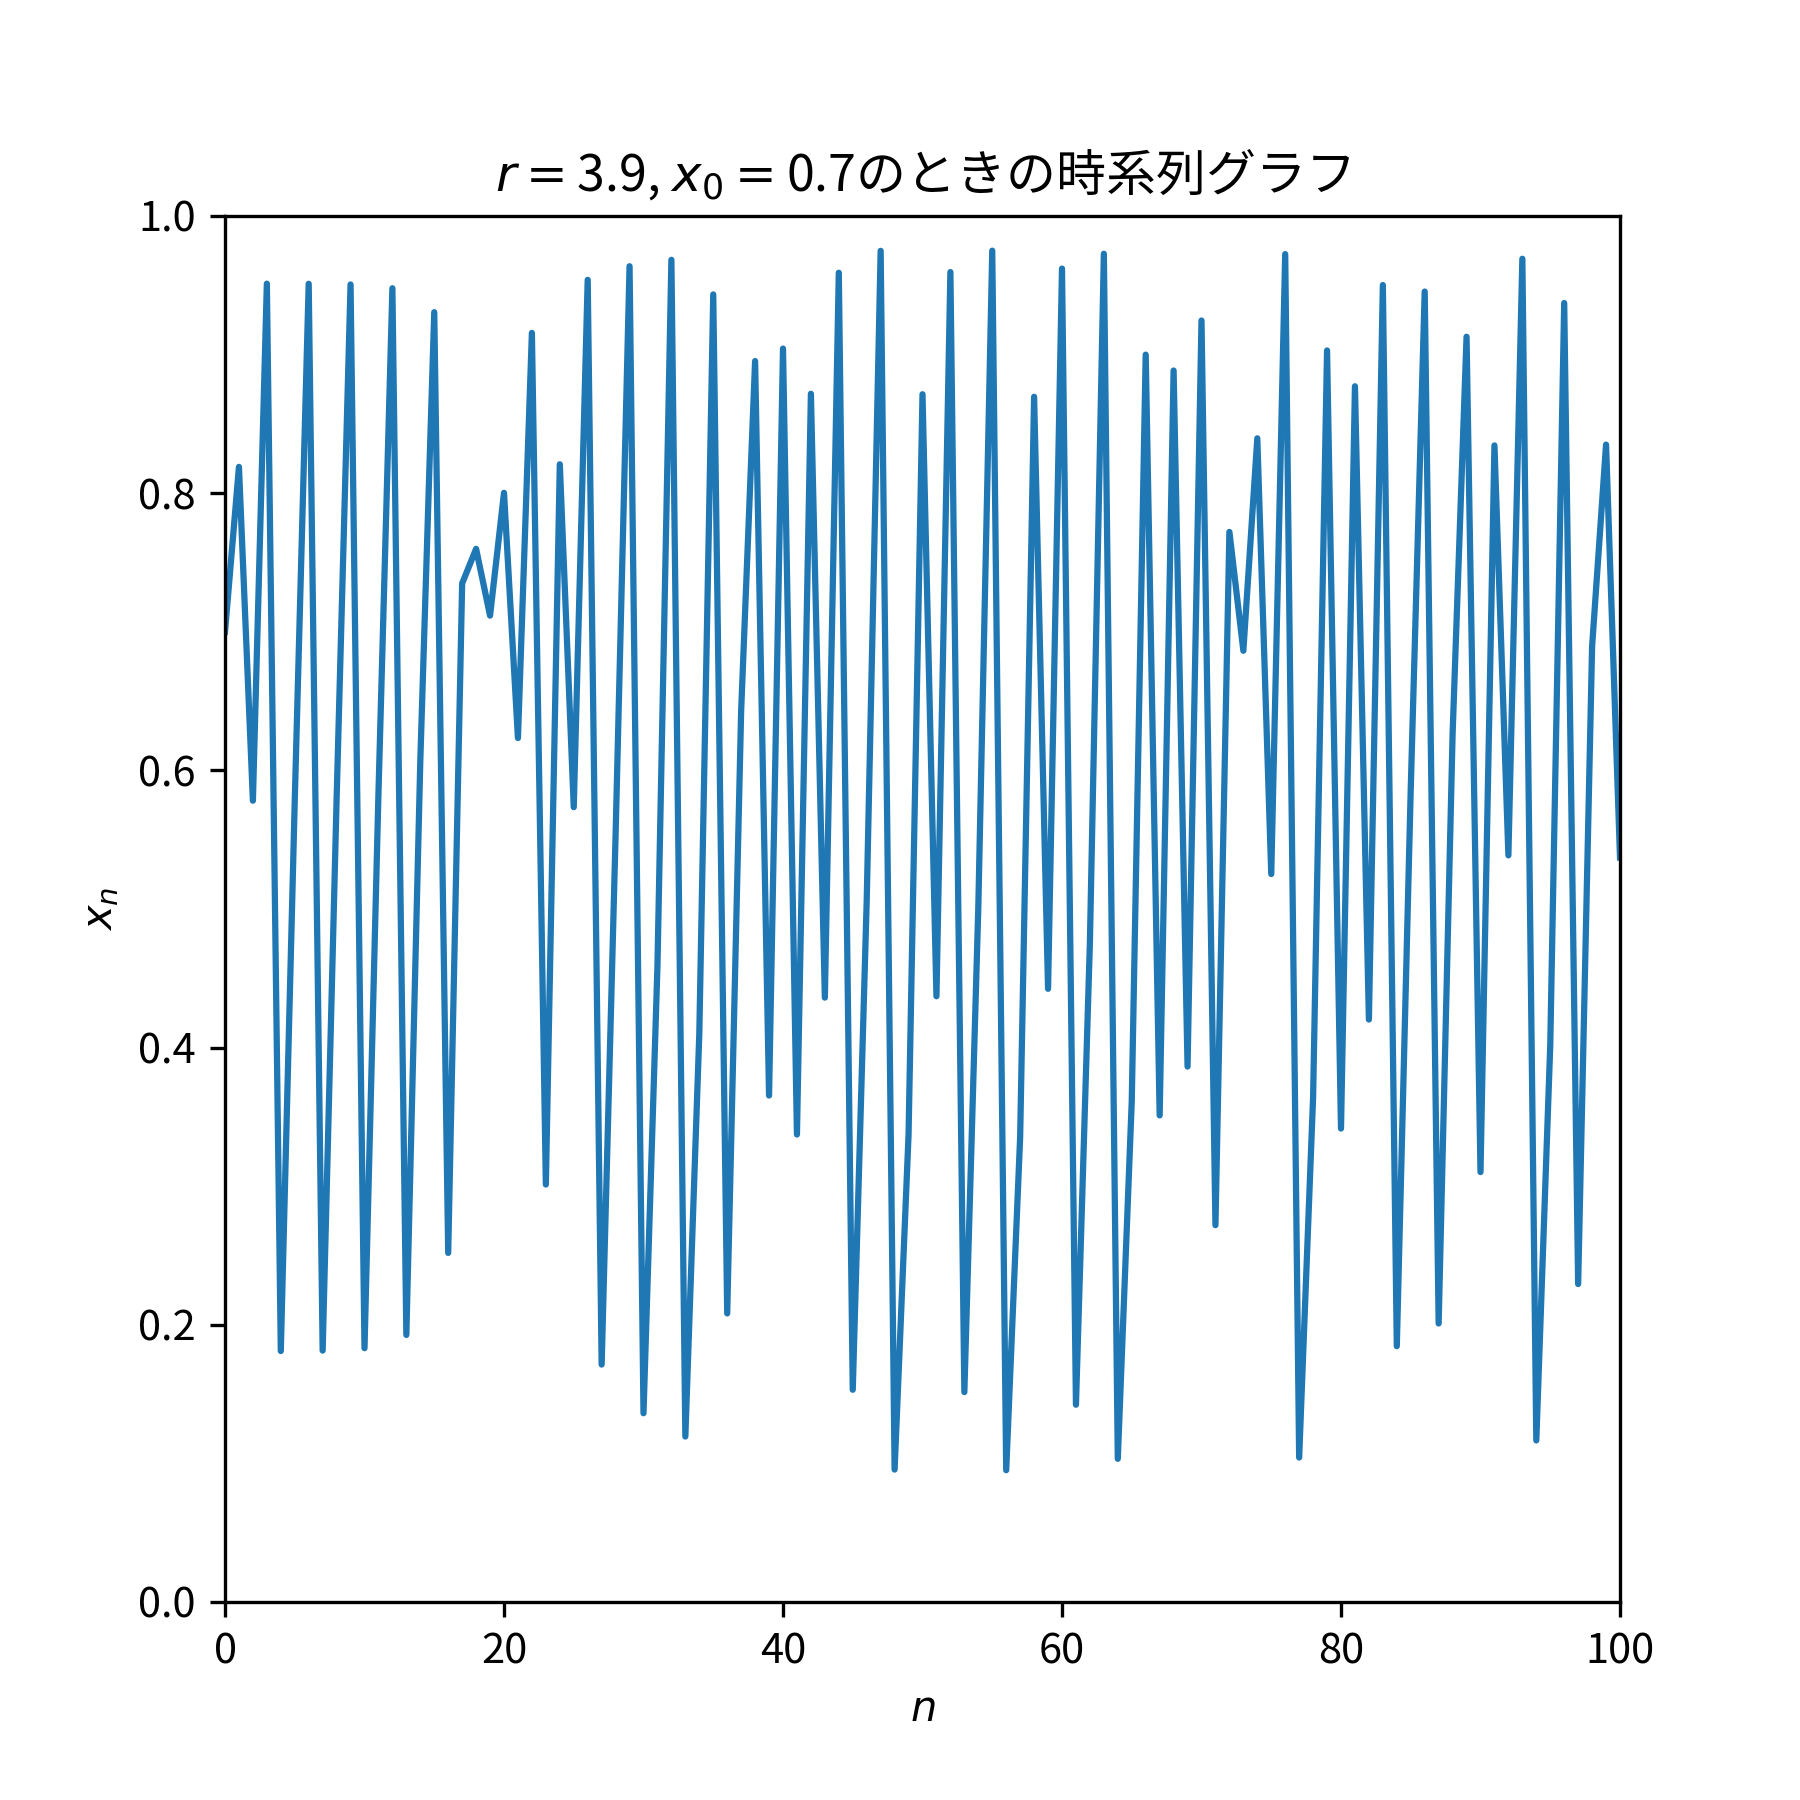
\includegraphics[keepaspectratio, scale=0.3]{images/Problem1/ctest2_6_1.png}
    \end{minipage}
  \end{tabular}
\end{figure}
結果:\\
時系列グラフは、ロジスティック回帰の各 $0 \leq n \leq 100$ のときの $x_n$ を計算しプロットしている。$x$ 軸は $n$ を、$y$ 軸には $x_n$ をとっている。この図から $r$ の値によって挙動が変わっているのが読み取れる。$r = 1.50, 2.60$ のときには $n$ を増加させていくと $x_n$ が収束していく。また、$r = 3.20, 3.50$ のときには $n$ を増加させていくと $x_n$ に周期性が見られるようになる。さらに、$r = 3.86, 3.90$ のときには $n$ を増加させていくと $x_n$ に周期性は現れることなく値が収束することもない。\\\\
考察:\\
この考察から、ロジスティック回帰は $r$ の値を変化させていくことでカオスの条件を満たす場合と満たさない場合があると考察した。\\


\subsection{課題2}
ロジスティク写像のリターンマップを描くためのプログラムを作成し、$r = 1.50, r = 2.60, r = 3.20,$ \\
$r = 3.50, r = 3.86, r = 3.90 のとき、x0 = 0.7$として個体数変動のリターンマッ
プを表示せよ。グラフには、$x_{n+1} = r(1 −x_n)x_n とx_{n+1} = x_n$ のグラフも表示すること。\\
画像:\\
\begin{figure}[htbp]
  \begin{tabular}{cc}
    \begin{minipage}[t]{0.45\hsize}
      \centering
      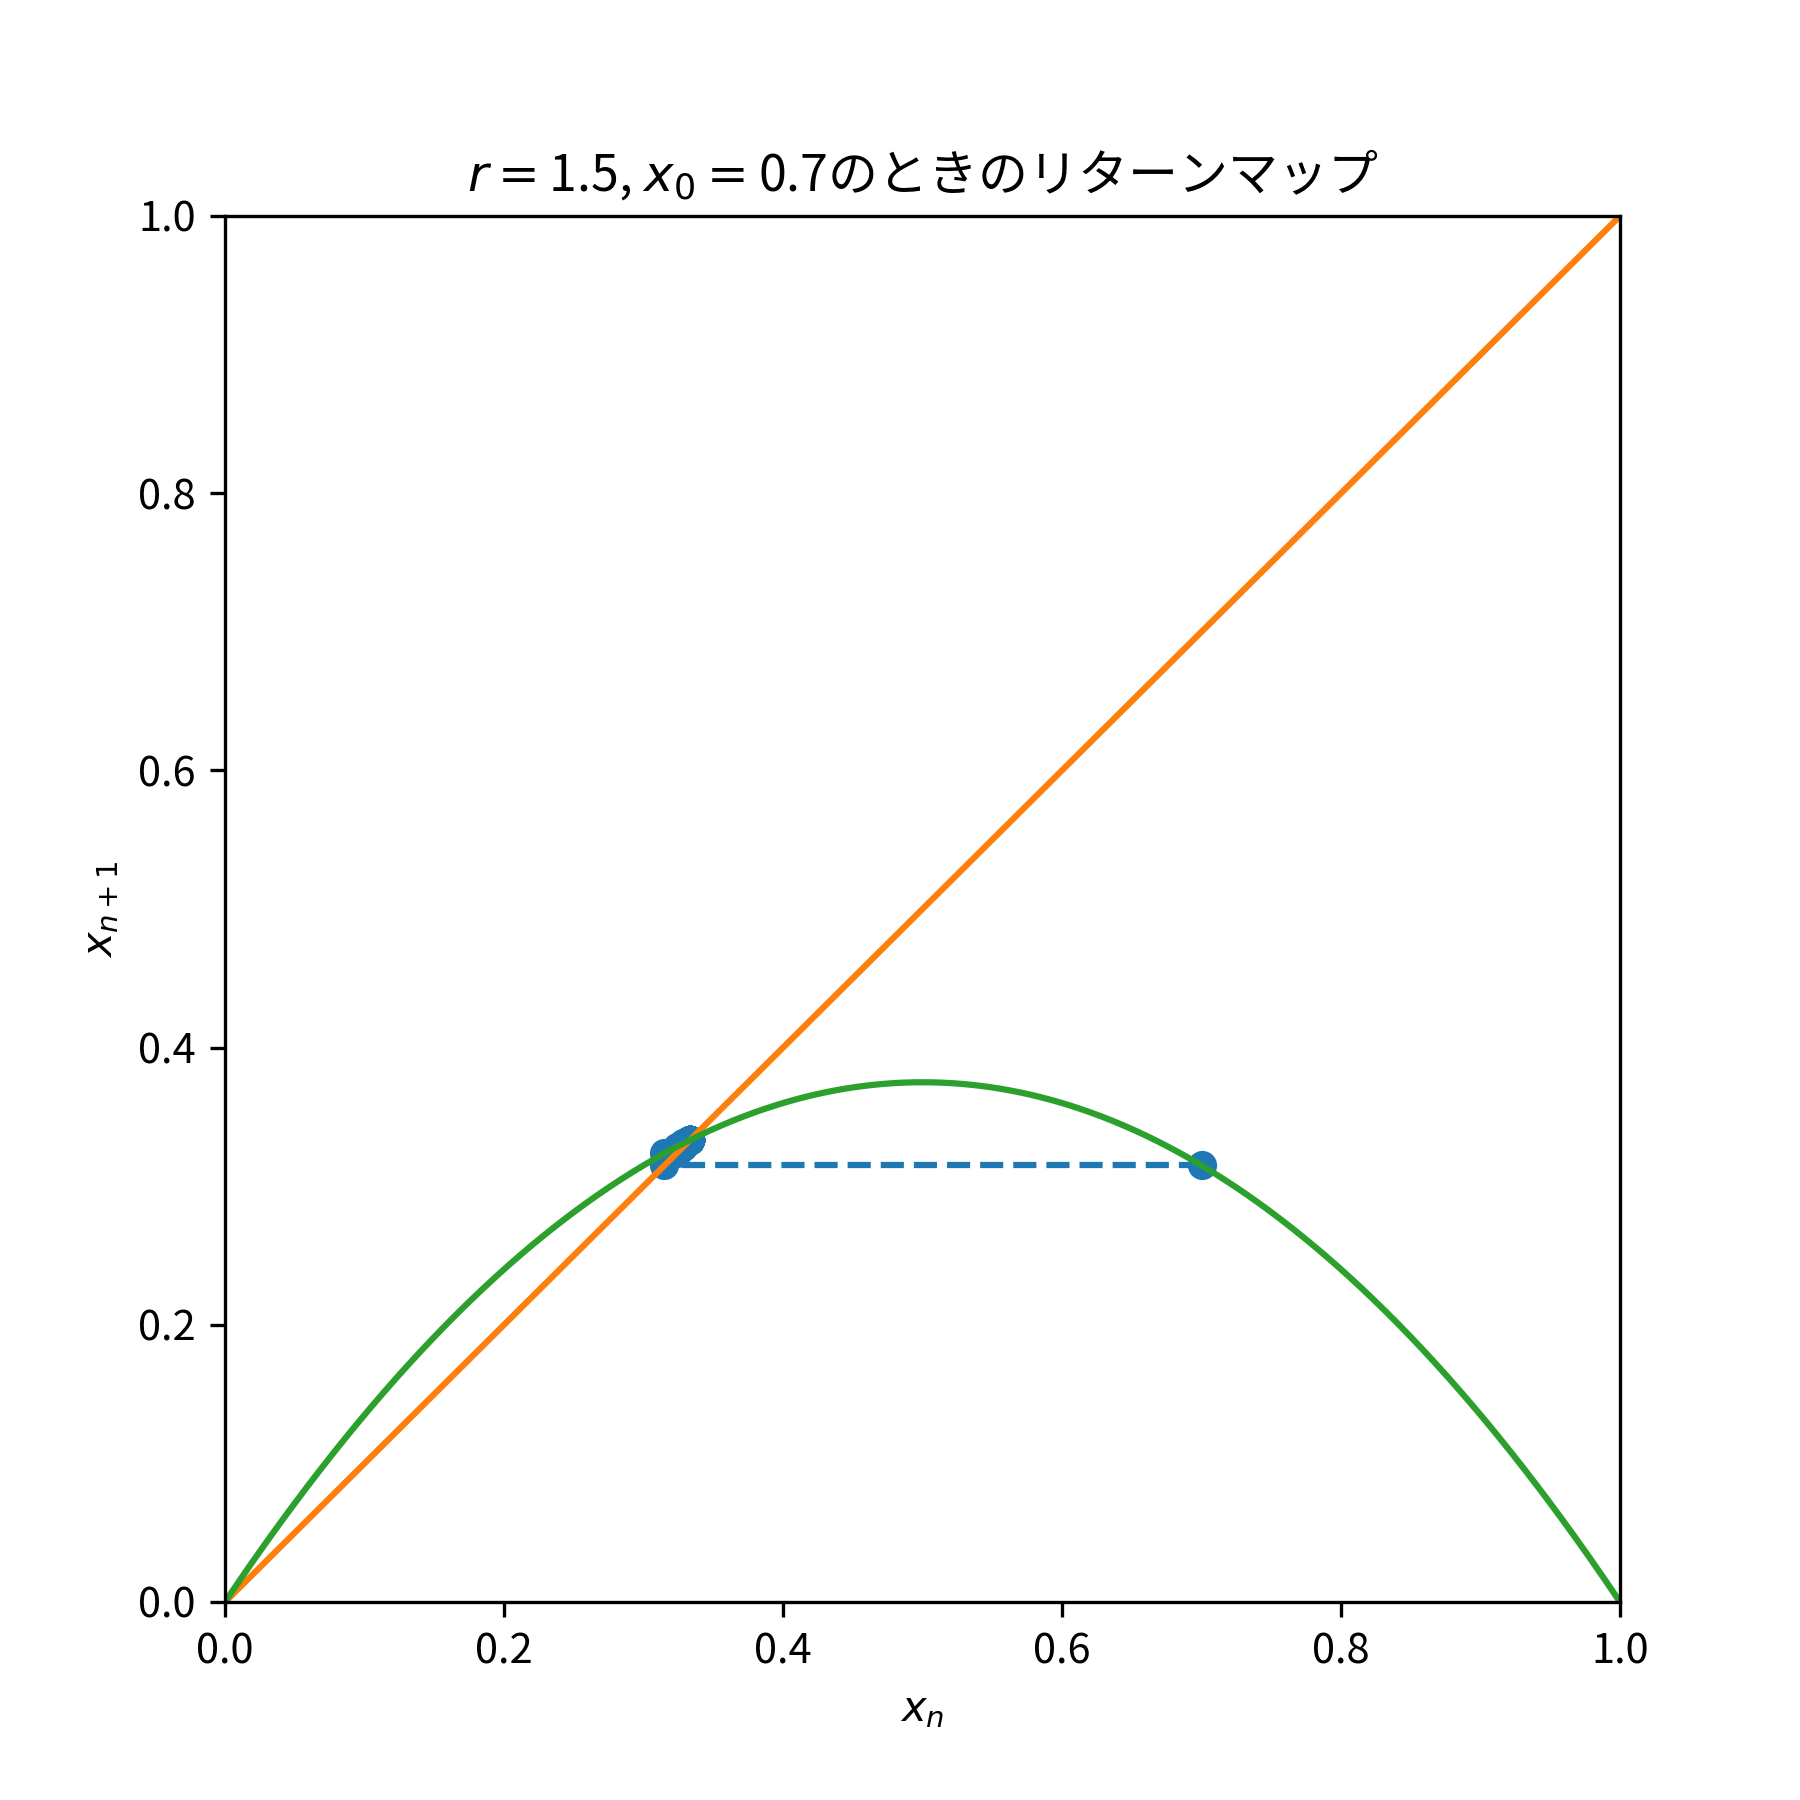
\includegraphics[keepaspectratio, scale=0.3]{images/Problem1/ctest2_1_2.png}
    \end{minipage} &
    \begin{minipage}[t]{0.45\hsize}
      \centering
      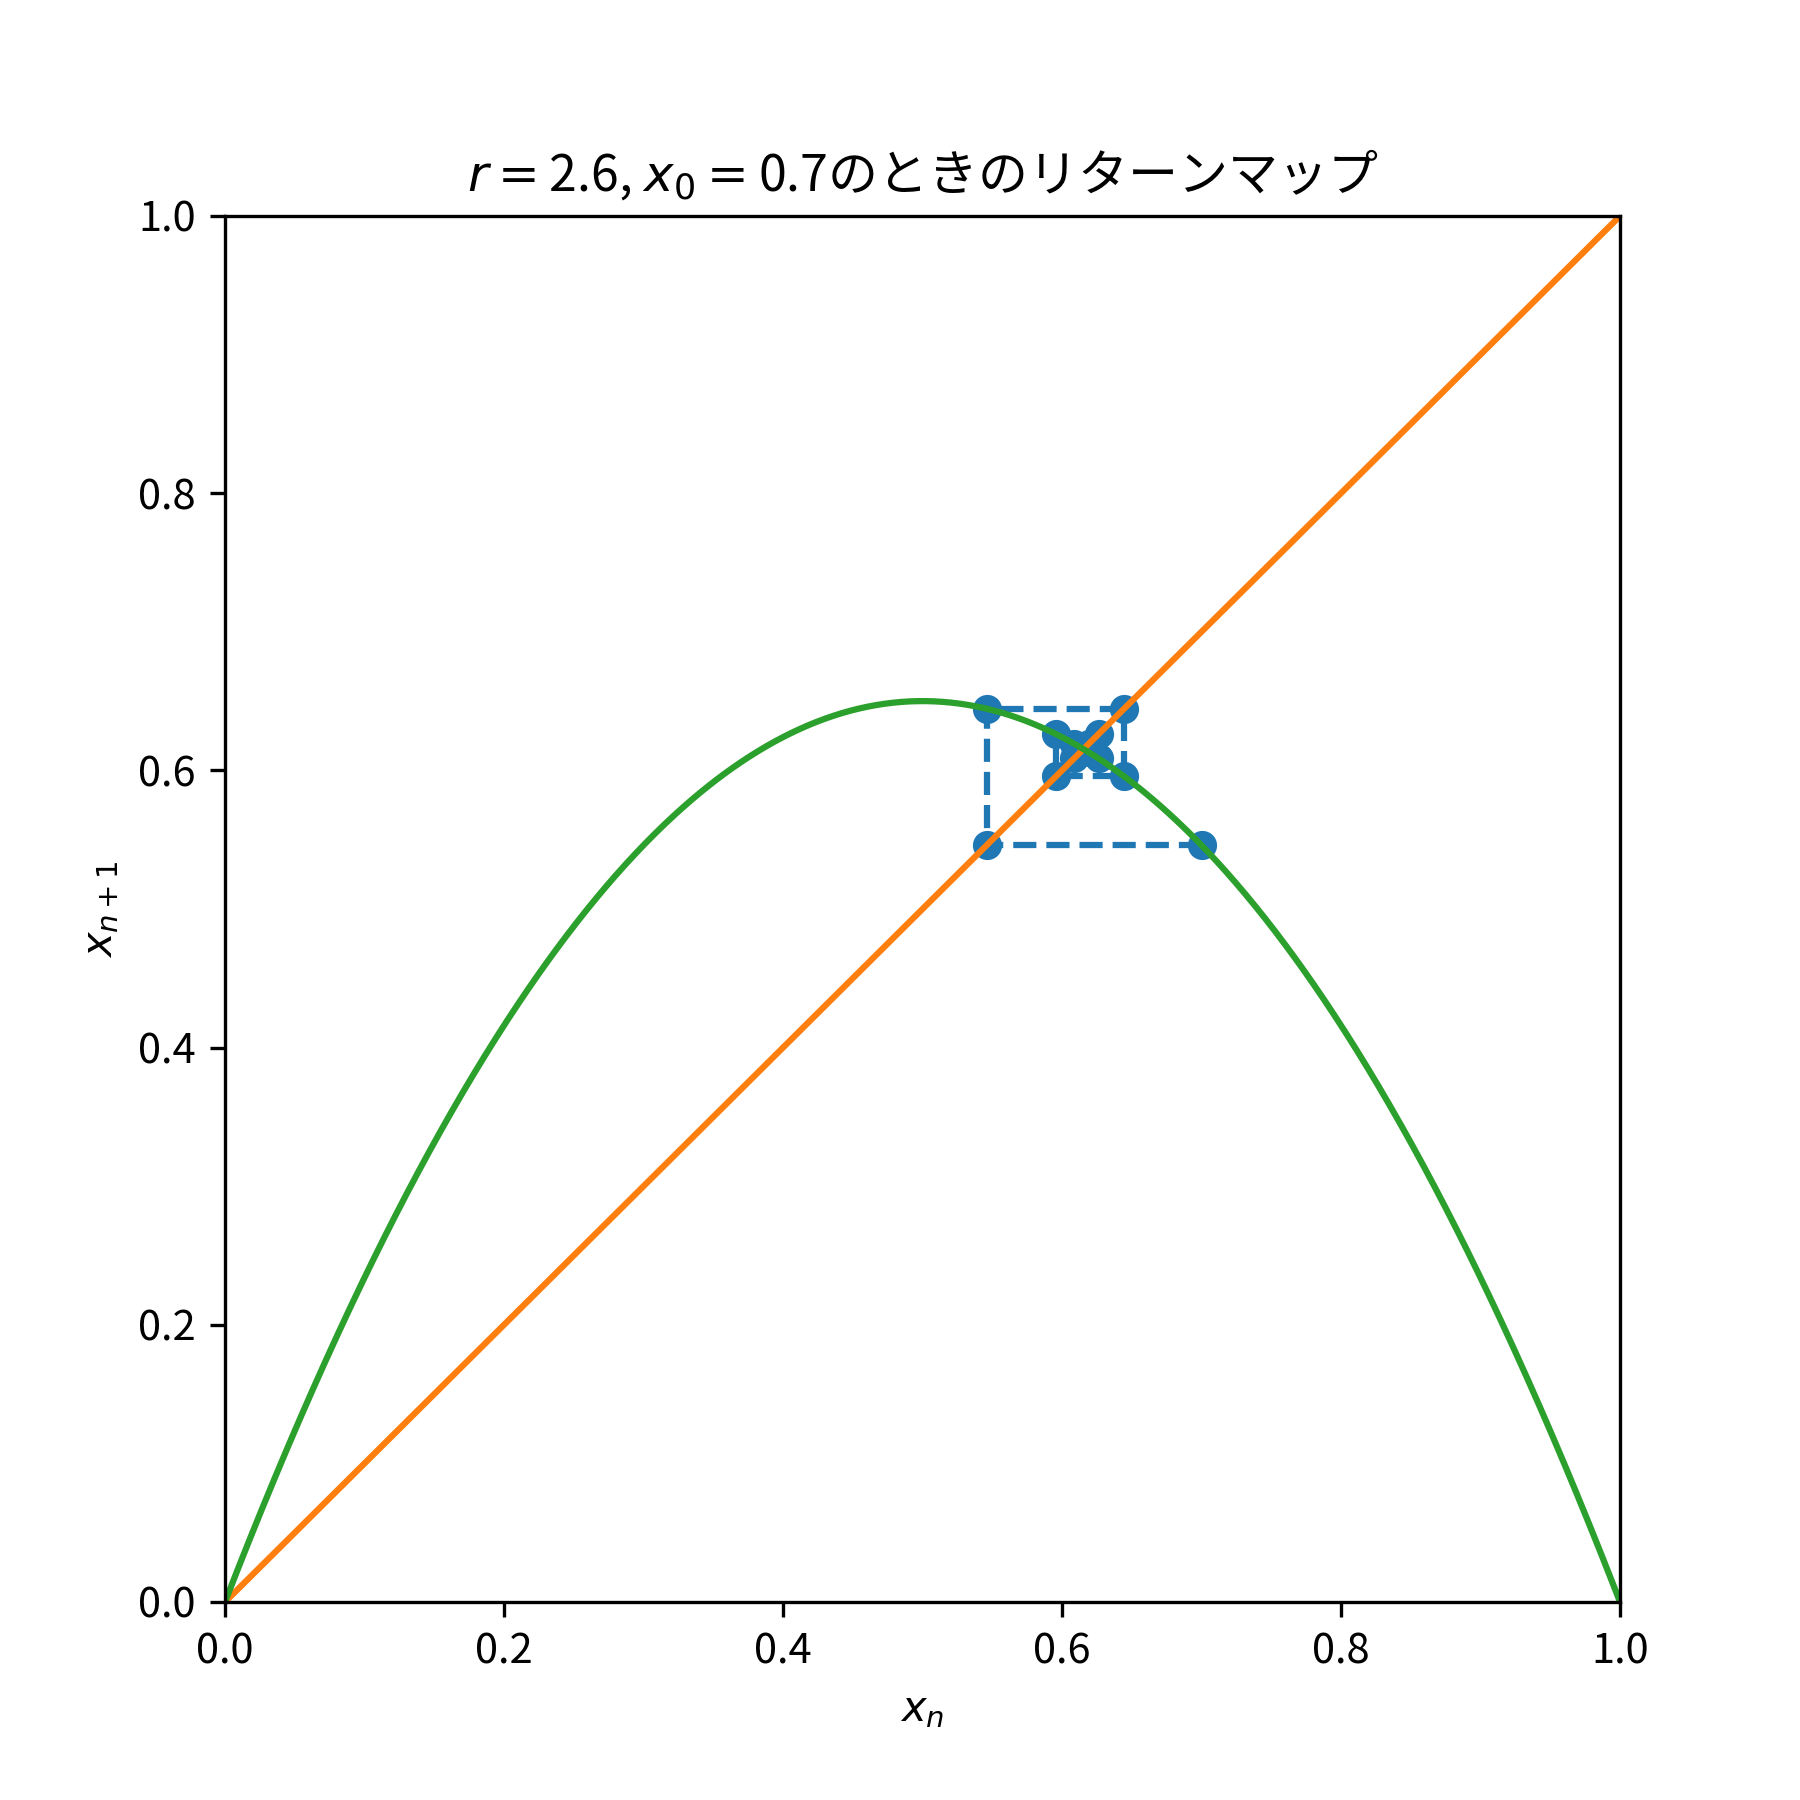
\includegraphics[keepaspectratio, scale=0.3]{images/Problem1/ctest2_2_2.png}
    \end{minipage} \\

    \begin{minipage}[t]{0.45\hsize}
      \centering
      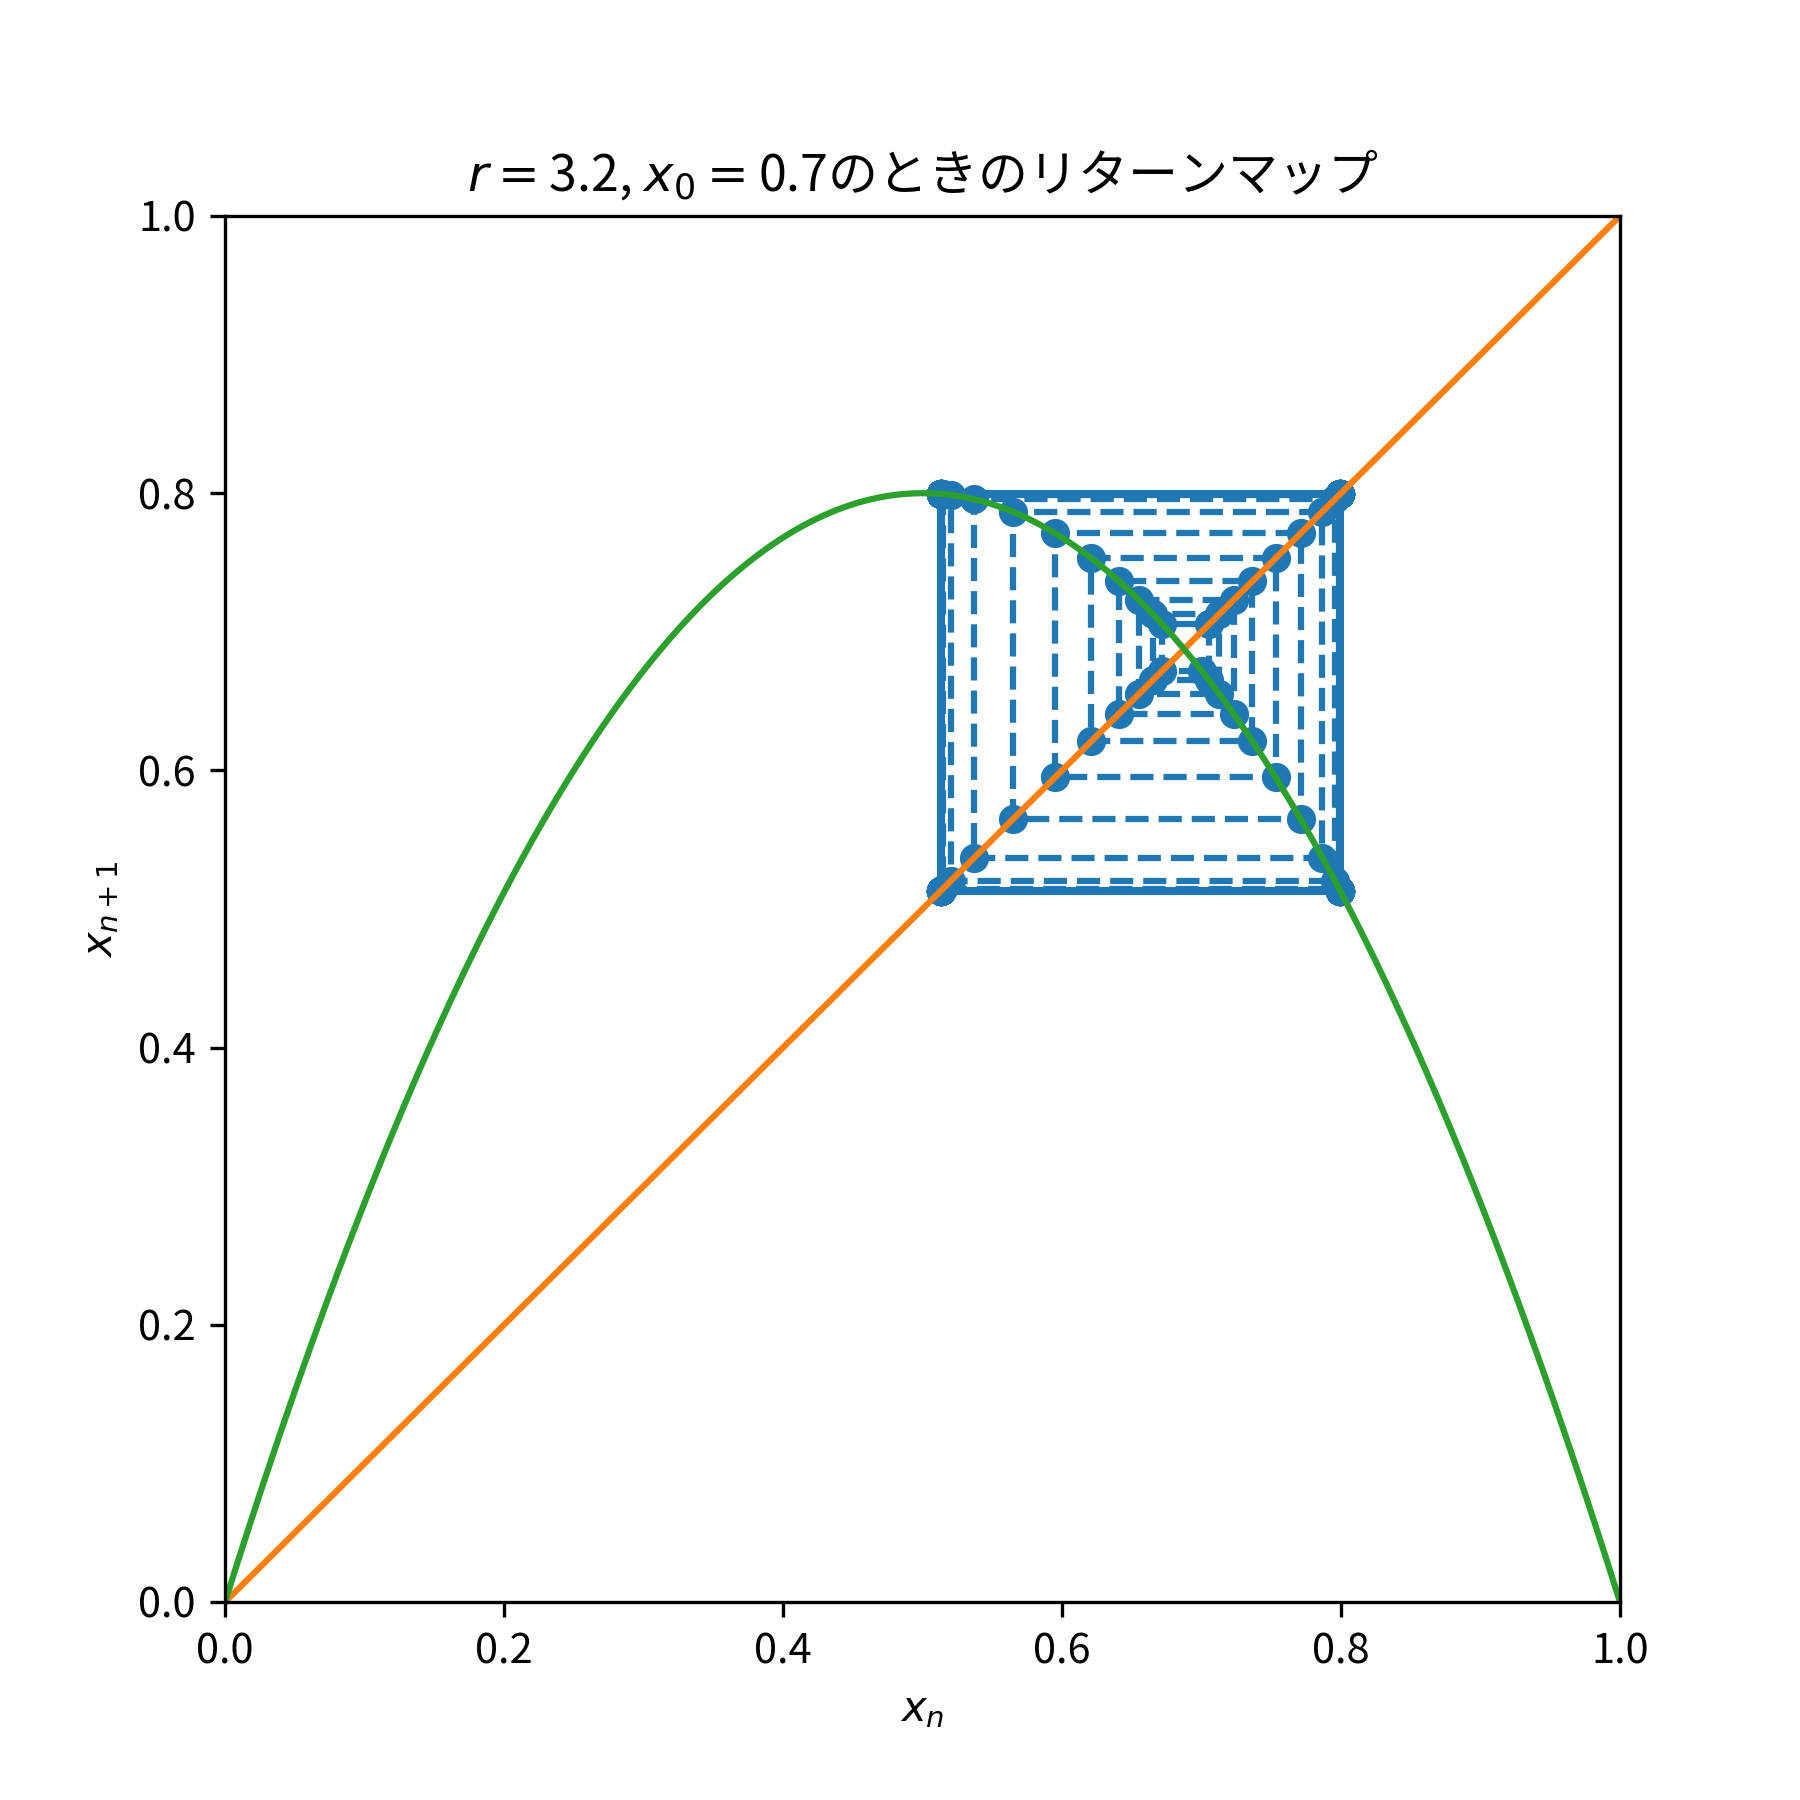
\includegraphics[keepaspectratio, scale=0.3]{images/Problem1/ctest2_3_2.png}
    \end{minipage} &
    \begin{minipage}[t]{0.45\hsize}
      \centering
      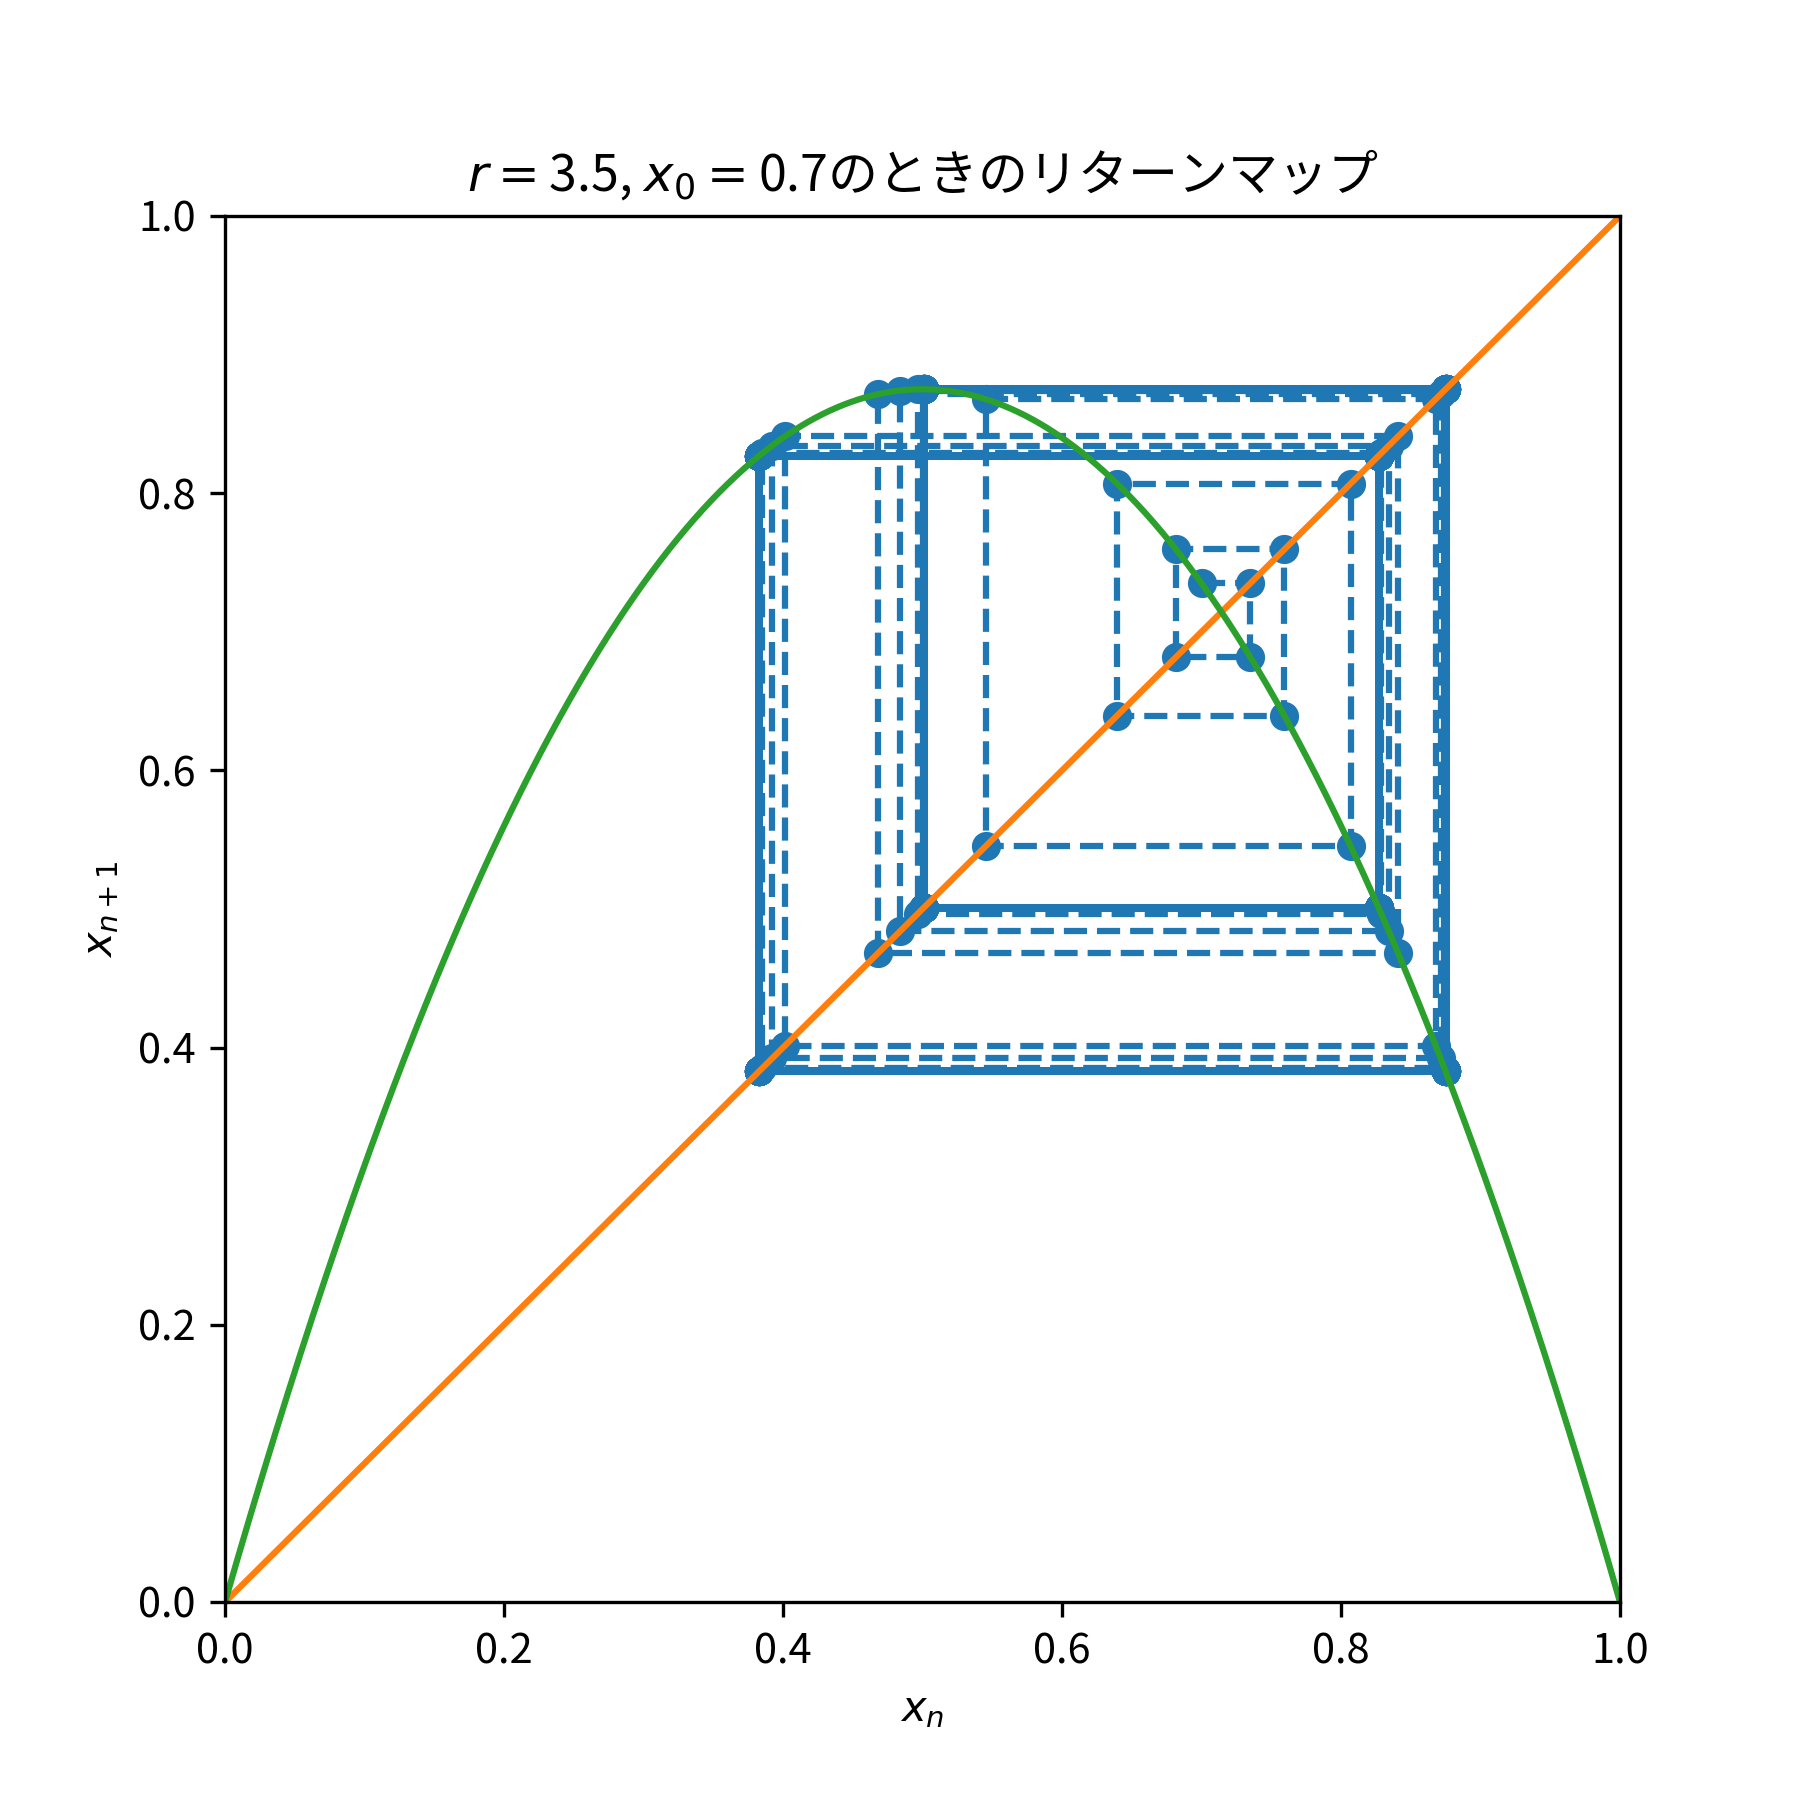
\includegraphics[keepaspectratio, scale=0.3]{images/Problem1/ctest2_4_2.png}
    \end{minipage} \\

    \begin{minipage}[t]{0.45\hsize}
      \centering
      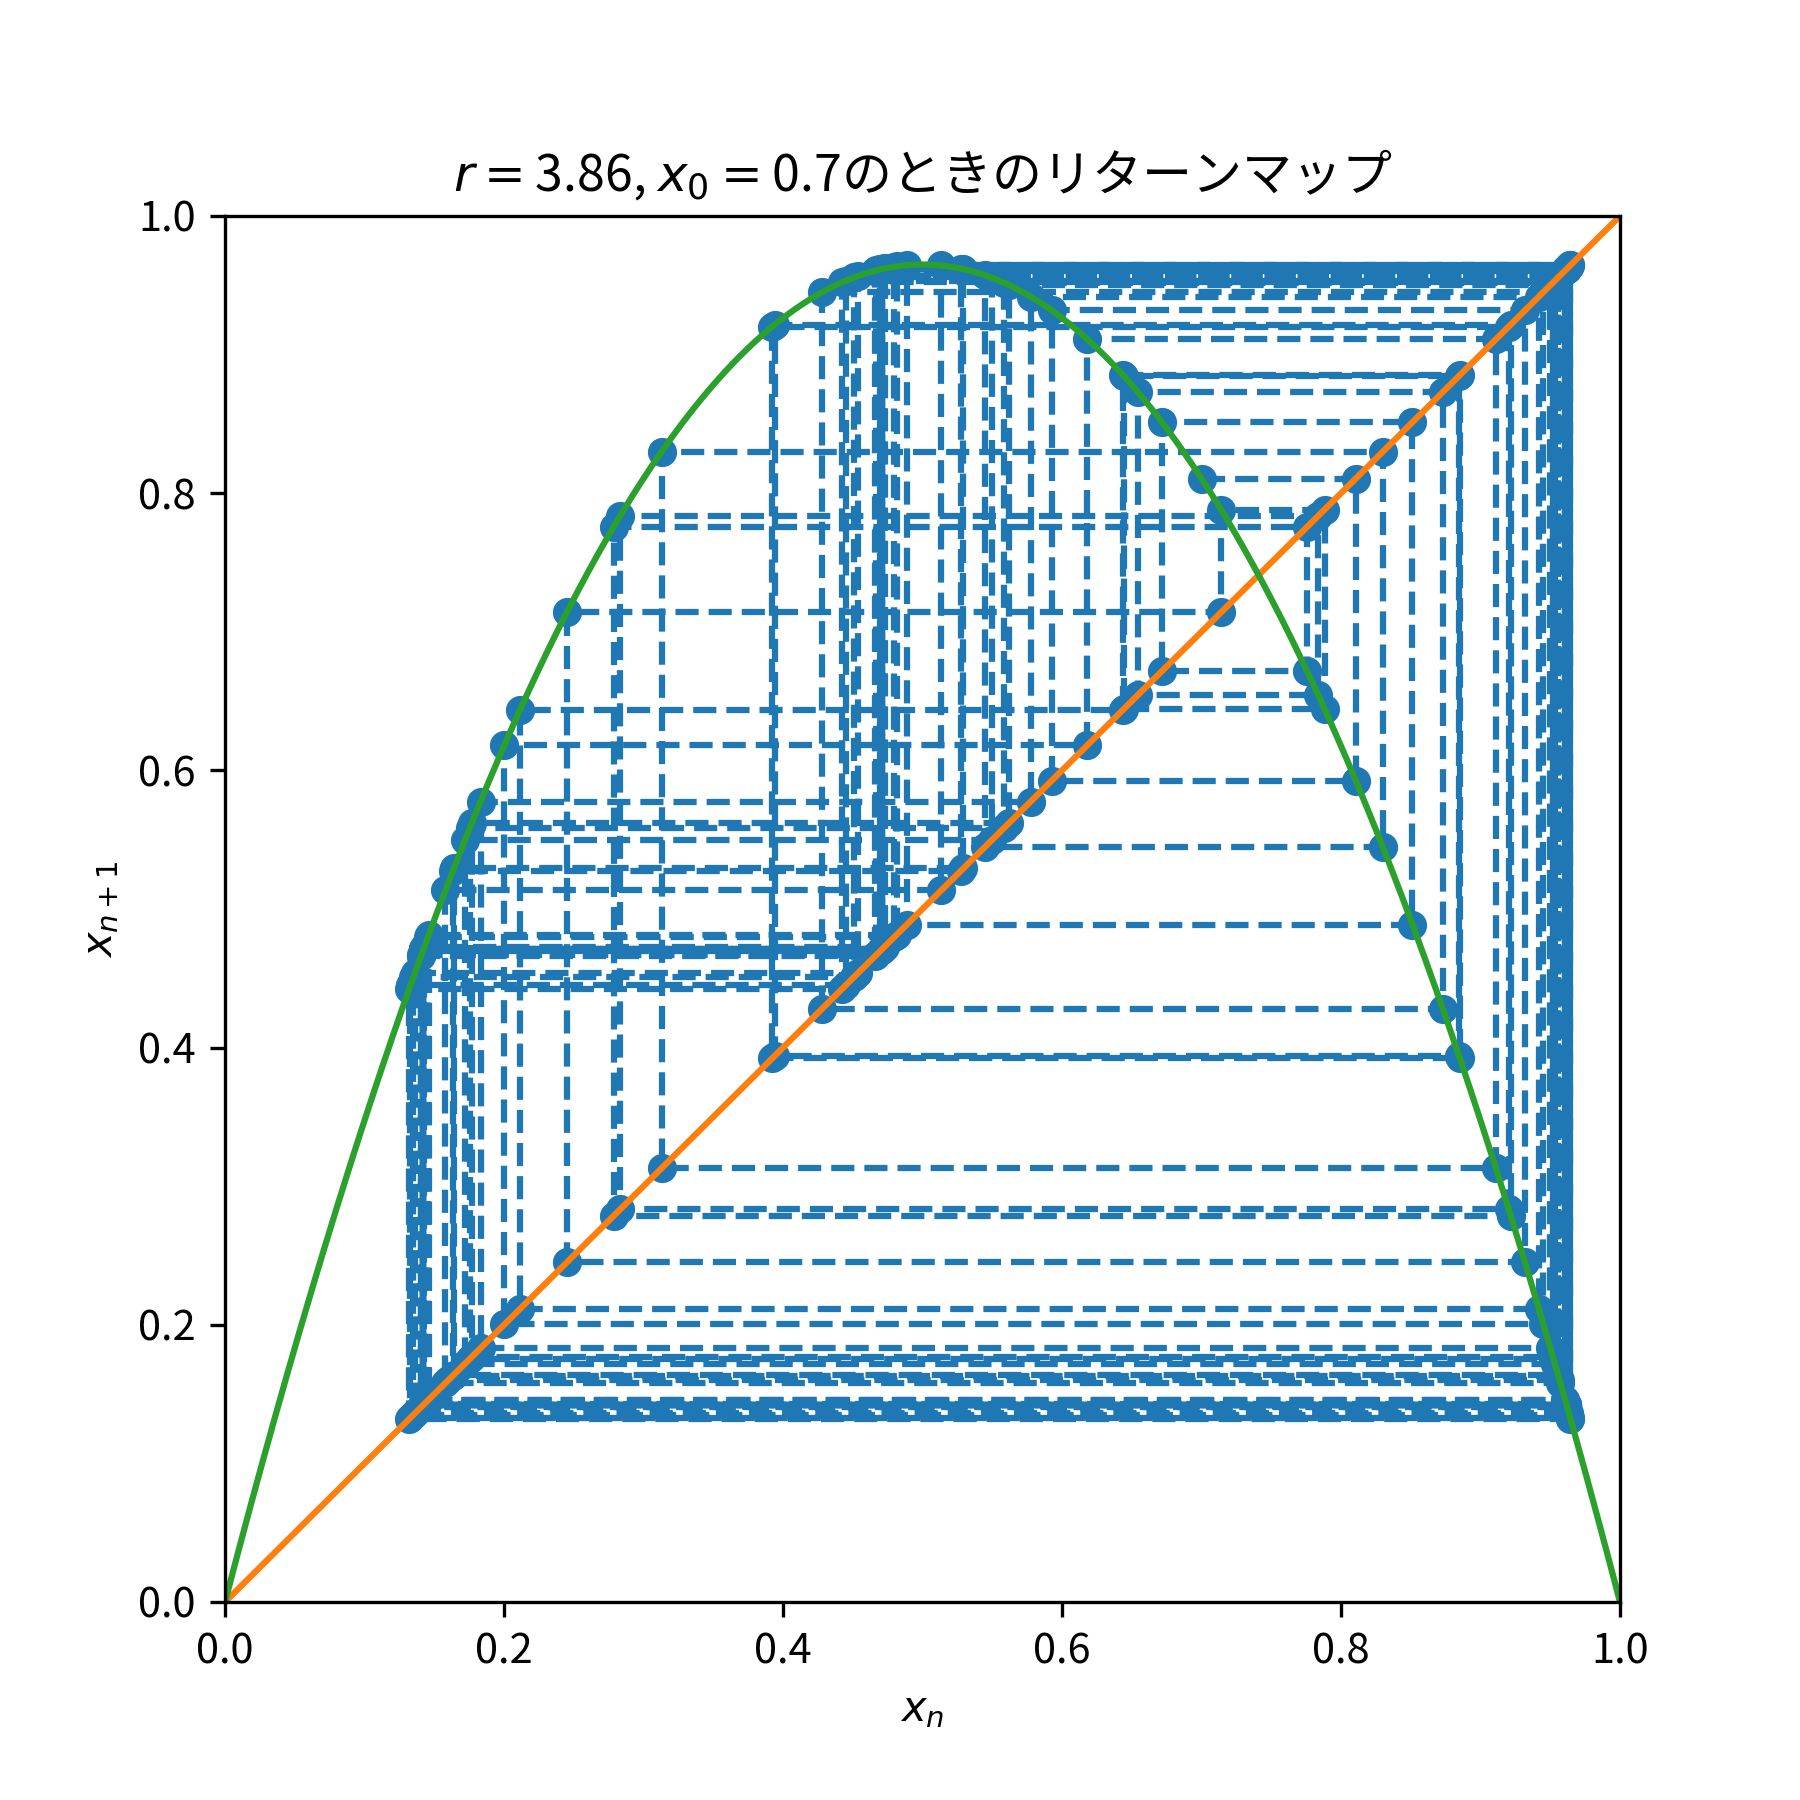
\includegraphics[keepaspectratio, scale=0.3]{images/Problem1/ctest2_5_2.png}
    \end{minipage} &
    \begin{minipage}[t]{0.45\hsize}
      \centering
      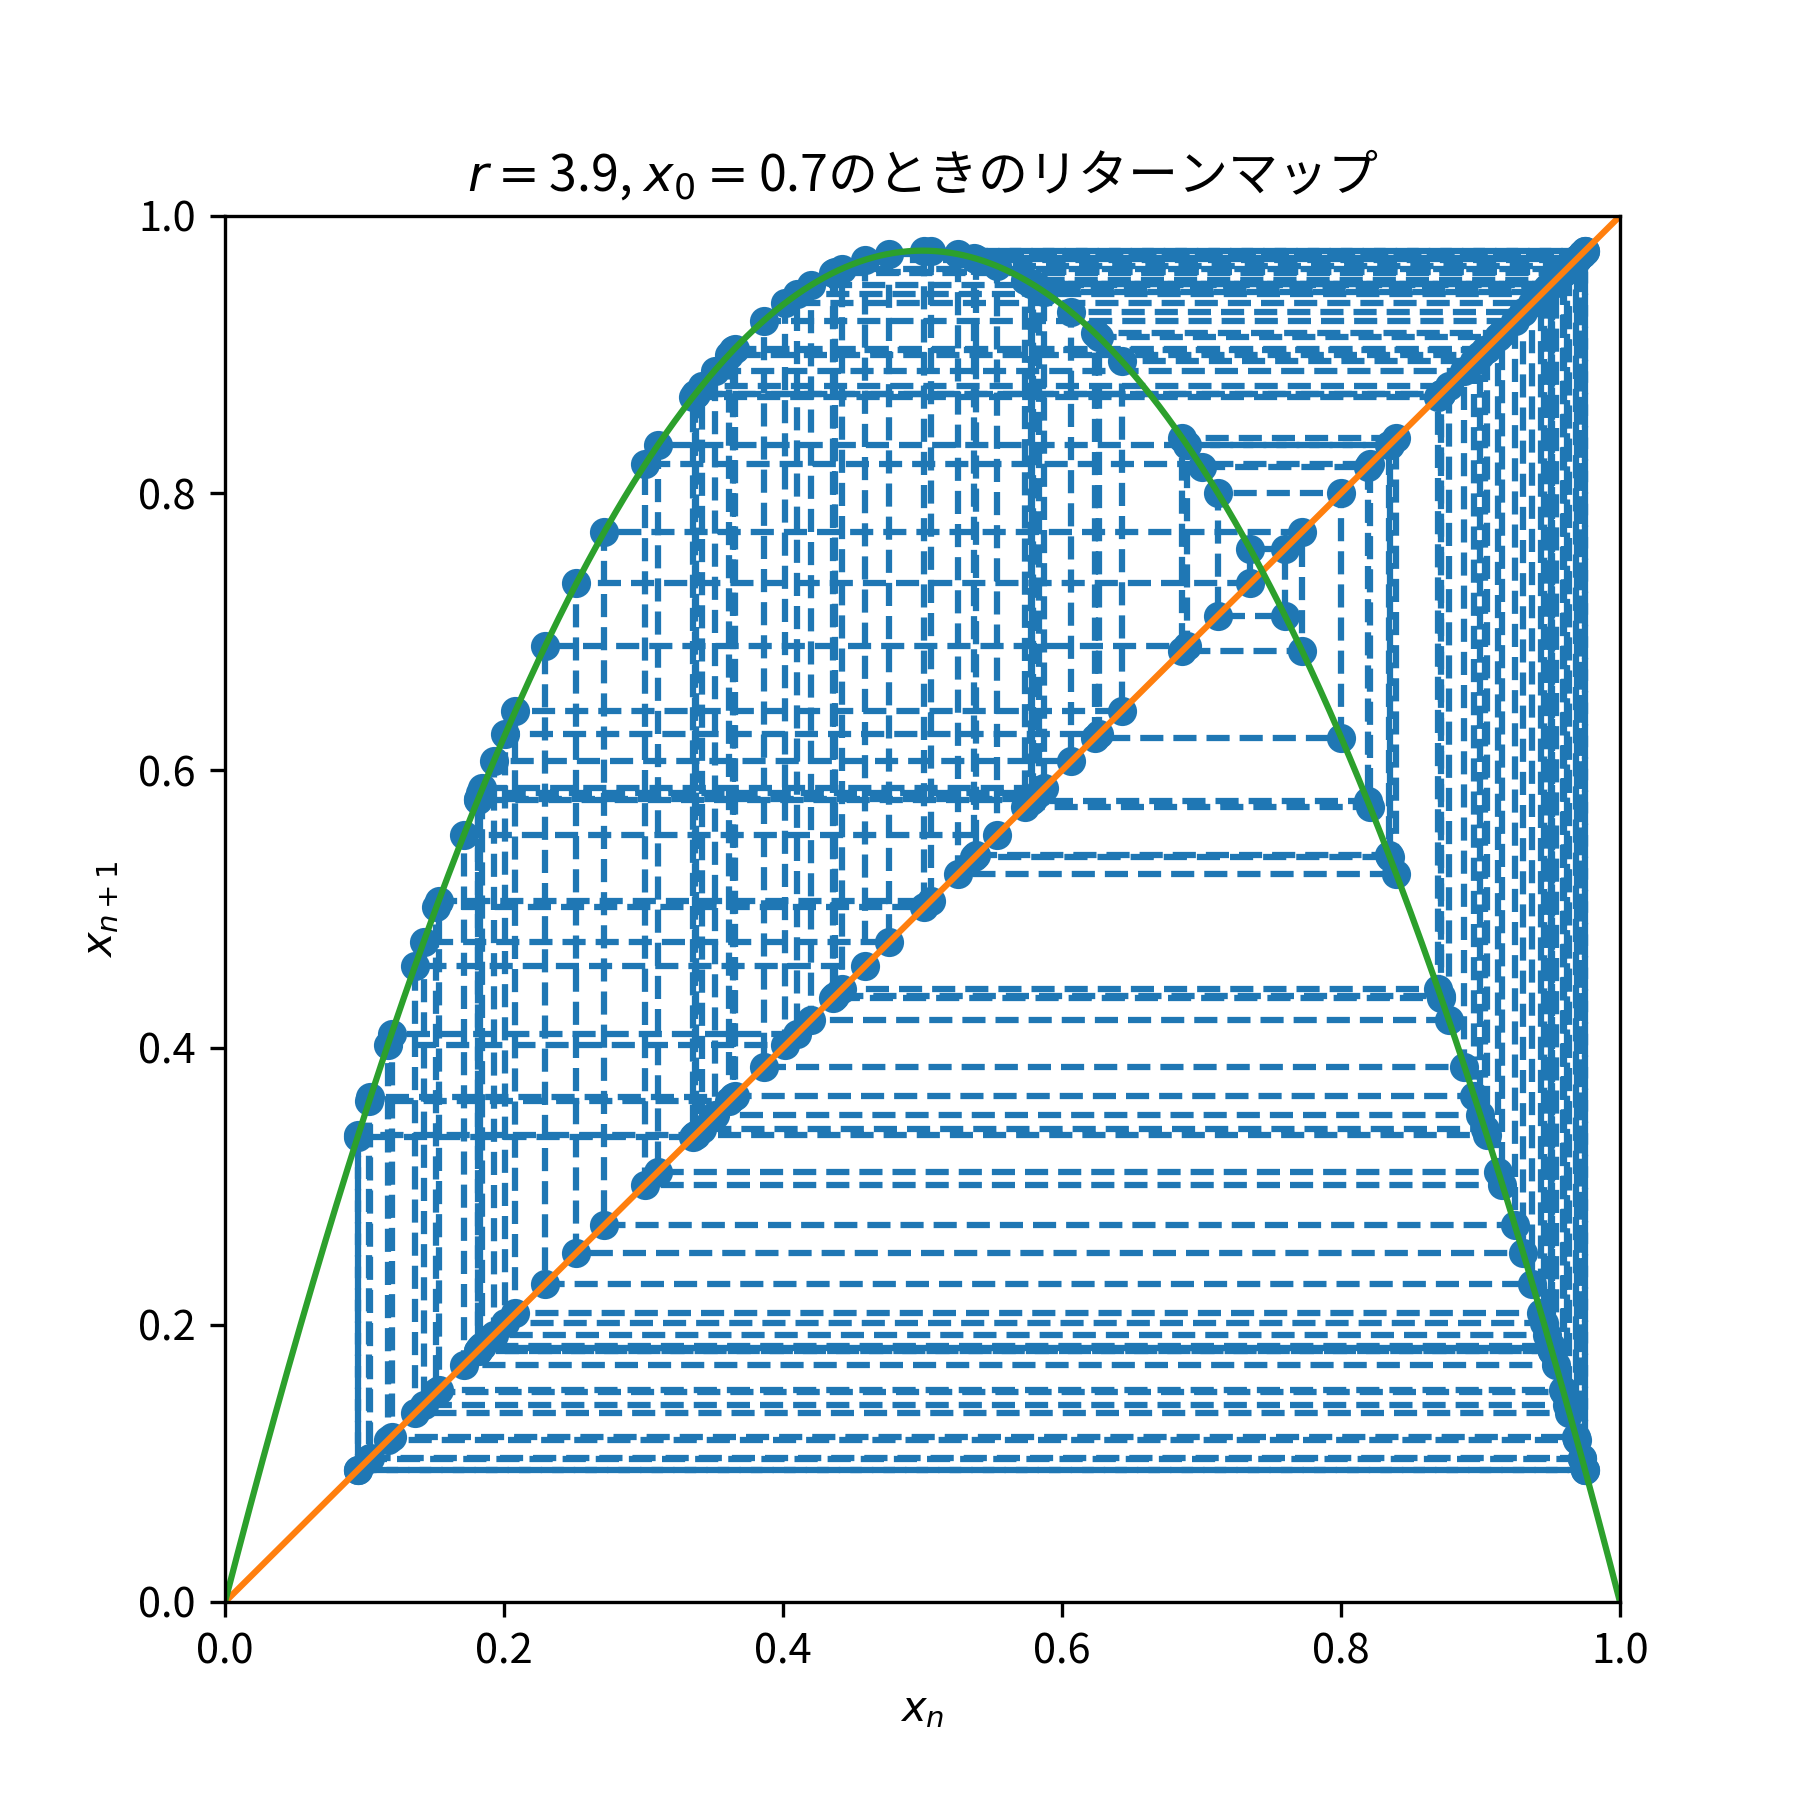
\includegraphics[keepaspectratio, scale=0.3]{images/Problem1/ctest2_6_2.png}
    \end{minipage}
  \end{tabular}
\end{figure}

結果:\\
リターンマップは、オレンジの線分が $x_{n+1} = x_n$ を示していて緑の線分が$x_{n+1} = r(1 −x_n)x_n$ を示している。時系列グラフをもとにリターンマップが描かれていくため、特徴としては似ている部分が多い。 $r = 1.50, 2.60$ のときは値が収束していき、その他では値が反復したり一切反復しないものなどがあり値は収束しない。\\\\

考察:\\
課題1, 課題2の結果から $x_{n+1} = r(1 −x_n)x_n$ と $x_{n+1} = x_n$、 $x_0$ の位置関係によって値が収束するかどうか、またカオスの状態かそうでないかが判断できるであろうと考察した。